\documentclass[paper=a4, parskip=half-]{scrartcl}
\usepackage[utf8]{inputenc}

\usepackage{amsmath}
\usepackage{mathtools}
\usepackage{marvosym} % for the \Lightning symbol
\usepackage{amssymb} % more icons/symbols
\usepackage{tablefootnote} % for footnotes in tables
% not in standard texlive, can't be asked to figure it out now
%\usepackage{ccicons} % creative commons icon
\usepackage{hyperref} % for hyper links
\usepackage[dvipsnames]{xcolor} % to color stuff -- dvipnames for additional color names
\usepackage[shortlabels]{enumitem} % to modify enumeration labels
\usepackage{tcolorbox} % for colored boxes - see https://tex.stackexchange.com/questions/66154/how-to-construct-a-coloured-box-with-rounded-corners/172608#172608
\usepackage{tikz} % drawing stuff
\usepackage{eurosym} % € (no, default LaTeX font doesn't include it)
\usepackage{natbib}
\usepackage{graphicx}

\usepackage{geometry}
 \geometry{
 a4paper,
 left=20mm,
 right=20mm,
 top=20mm,
 bottom=30mm,
 }


\title{Security of Wireless Networks}
\author{\texttt{\{thgoebel\}@ethz.ch}}
\date{ETH Zürich, HS 2020}

% Custom commands
\newcommand{\setzeroone}{\lbrace 0, 1 \rbrace} % => {0,1} (Notice the missing $$)
\newcommand{\horizontaldivider}{\begin{center} \line(1,0){350} \end{center}}

\begin{document}

\begin{titlepage}
\maketitle
\vspace{5cm}
\thispagestyle{empty}


\begin{abstract}
This is a summary for the course \textit{Security of Wirless Networks (SOWN)} at ETH Zurich.

This summary is created during the autumn semester 2020.
But due to the few changes in syllabus content in the past we have reason to believe that it is also relevant beyond that very semester.

We do not guarantee correctness or completeness, nor is this document endorsed by the lecturers.
Feel free to point out any erratas.
\end{abstract}

\end{titlepage}

\tableofcontents
%\listoffigures
%\listoftables
\newpage


\section{Wireless Basics}

\begin{figure}[h]
	\centering
	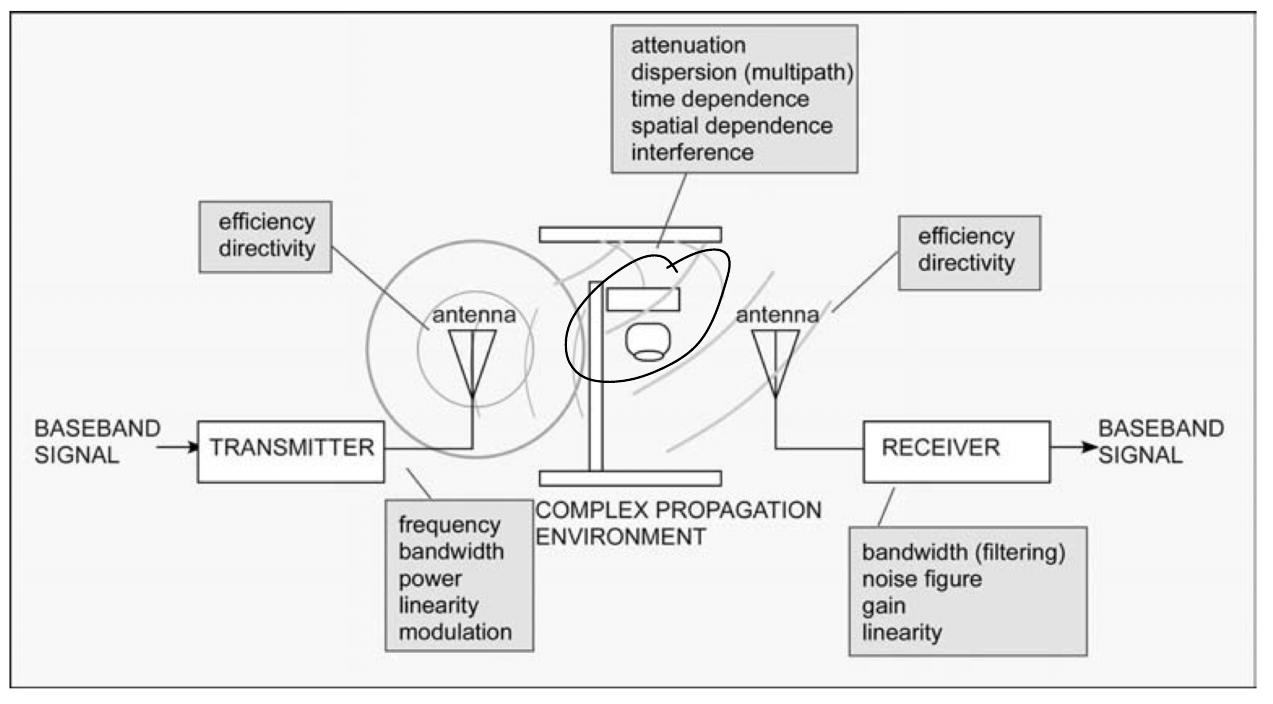
\includegraphics[scale=0.4]{images/1-wireless-system.png}
	\caption{A wireless system, its basic components and characteristic measures}%
	\label{fig:wireless-system}
\end{figure}

\paragraph{Radio Frequency Signal}
Electromagnetic radiation, with waves being created in the antenna by an
alternating current at the desired frequency. Mathematically described as a
function of the time $t$:
\[ v(t) = A \sin (2 \pi f t + \phi) \]
with amplitude $A$, frequency $f$ and phase $\phi$. Also recall that the period
is $T = \frac{1}{f}$ and the wavelength (distance traveled during one period)
is $\lambda = \frac{v}{f}$ (usually $v=c$ speed of light).

\paragraph{Bandwidth}
The capacity of a communications link to transmit the maximum amount of data
from one point to another over a connection in a given amount of time (in bits
per second bps). An analogy: The amount of water that can flow through a water
pipe.

In other words, the measure of frequency content of the signal. E.g.\ the human
voice contains frequencies in the range from 30 Hz to 10 kHz, and the bandwidth
of a single 802.11 channel is 22 MHz.

Note that often the bandwidth of the base-band and that of the carrier (and
thus that of the modulated signal) differ! E.g.\ see spread spectrum techniques
(\autoref{sec:jamming-resistant-comm}). Low variability of the signal in time
corresponds to a small bandwidth, whereas a high variability corresponds to a
large bandwidth

\begin{figure}[h]
	\centering
	
\includegraphics[scale=0.35]{images/1-wifi-channels.png}
	\caption{2.4 GHz WiFi Channels \href{https://en.wikipedia.org/wiki/List\_of\_WLAN\_channels\#/media/File:2.4\_GHz\_Wi-Fi\_channels\_(802.11b,g_WLAN).svg}{[Source]}}%
	\label{fig:wifi-channels}
\end{figure}

\paragraph{Baseband}
An original transmission signal that has not been modulated or has been
demodulated to its original frequency, aka the actual \textbf{information
	signal}. Most telecommunication protocols require base-band signals to be
converted, or modulated, to a higher frequency in order to be transmitted over
long distances.

\paragraph{Carrier}
A transmitted electromagnetic pulse or wave at a steady base frequency of
alternation on which information can be imposed. Typically \textbf{a pure
	sinusoid of a particular frequency and phase} that will carry the information.
Usually the frequency of the carrier is much higher than that of the baseband.
To go from baseband to passband, we need to multiply the analytic signal with a
carrier, where $f_c$ is the carrier frequency and $a(t)$ is the amplitude.
\[ x_{RF} (t) = \Re \{a(t)e^{i\theta (t)}\} = a(t) \cos (2 \pi f_c t + \theta(t))\]

\subparagraph{Upconversion}
This process is called \textbf{up-conversion}, and it's necessary mainly for
two reasons: to enable simultaneous transmission of different signals by using
a different carrier frequency (for each transmission) and to transform a
complex signal into a real one, since only real signals can actually be
transmitted. At the receiver, it's then down-converted such that the subsequent
processing can be done in the complex-valued baseband domain.

In order to actually perform the up-conversion, we need an oscillator to
produce the cosine wave at the chosen (carrier) frequency and a mixer to
multiply it with the baseband signal, producing the frequency shift.

\paragraph{Modulated Signal}
A carrier that has been loaded or modulated with the information signal.

\paragraph{Modulation}
Process of imposing the baseband onto the carrier. The baseband is used to
alter one aspect of the carrier, such as: signal strength (\textit{amplitude
	modulation AM}), frequency (\textit{frequency modulation FM}), phase
(\textit{phase modulation PM}). In other words, one of the values $A, f, \phi$
in the above equation of the signal is manipulated.

\paragraph{Amplitude-shift keying ASK}
Modulation technique varying the amplitude of the signal.

\paragraph{Frequency-shift keying FSK}
Modulation technique varying the frequency of the carrier.

\paragraph{Phase-shift keying PSK}
Modulation technique varying the phase of the carrier. It's used, for example,
in WiFi, RFID, Bluetooth. Specific versions include Binary PSK, Quadrature PSK
and Differential PSK.\@ Example: if the baseband bit is 0 do nothing to the
carrier, if it is 1 shift the carrier phase by $\pi$.

\paragraph{On-Off-Keying OOK}
Simple form of amplitude-shift keying ASK.\@ Represents data as the presence
(1) or absence (0) of a signal. E.g.\ Morse code.

\paragraph{I-Q Signal Representation}
A pair of periodic signals are said to be in `quadrature' when they differ in
phase by 90 degrees (e.g.\ the sine and cosine wave). The `in-phase' or
reference signal is referred to as `I' (conventionally cosine), and the signal
that is shifted by 90 degrees (in quadrature) is called `Q' (conventionally
sine). It's used to represent modulations.
\[ I(t) = a(t) \cos (\phi(t)) \leftarrow  \textrm{Analytic signal, } a(t) \textrm{ is the amplitude}\]
\[ Q(t) = a(t) \sin (\phi(t)) \]

\paragraph{Antenna}
Interface between radio waves in the air and electric alternating currents in a
conductor. Types include: omni/dipole, yagi, horn, can-tenna.

The directionality of an antenna described how well it transmits/receives into
a particular direction.
\begin{itemize}
	\item \textbf{isotropic} --- Theoretical, radiates with the same intensity equally in all directions. Often used as a reference antenna when calculating the gain.
	\item \textbf{omnidirectional} --- Radiates equally well in all directions in a flat horizontal plane. Most common types in consumer devices.
	\item \textbf{directional} --- Radiates best in a given direction by focussing its power. Can thus work with weaker signals than an omnidirectional antenna of the same power.
\end{itemize}

\begin{figure}[h]
	\centering
	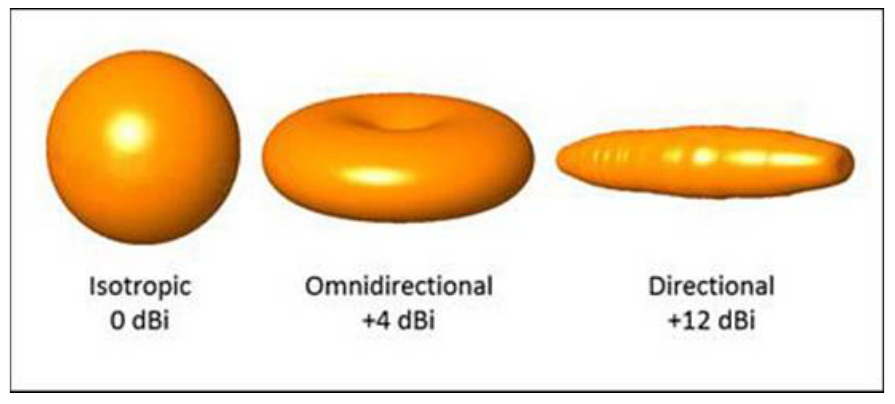
\includegraphics[scale=0.4]{images/1-directionality.png}
	\caption{Antenna directionality}%
	\label{fig:directionality}
\end{figure}

\paragraph{Phased Array}
Array of fixed antennas where the phase of each signal is dynamically adjusted
so that the signal will be in phase when viewed from a given direction. Allows
\textit{beam steering} towards a specific direction. Possible applications? Can
it be used to achieve security (e.g.\ confidentiality)?

\begin{figure}[h]
	\centering
	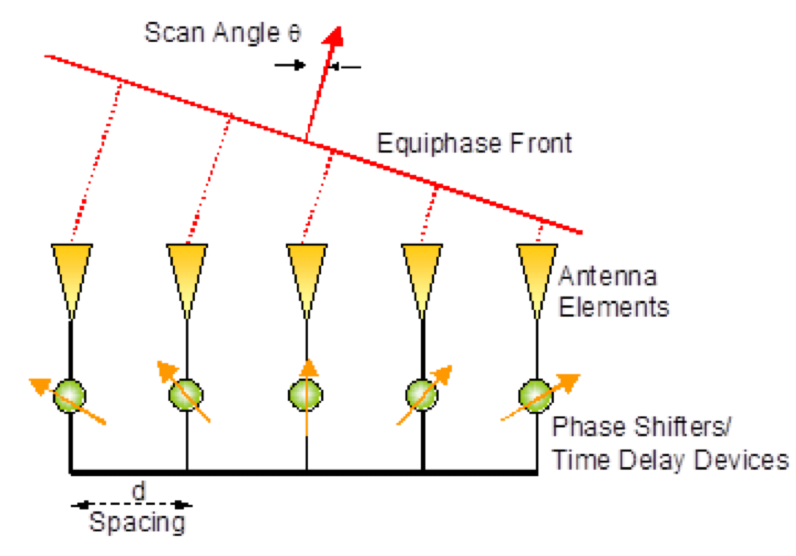
\includegraphics[scale=0.4]{images/1-beam-steering.png}
	\caption{Beam steering}%
	\label{fig:beam-steering}
\end{figure}

\paragraph{Transmitter/Receiver}
Converts from digital to analogue, applies modulation and connects to the
antenna (and vice versa). Properties: transmitted power, carrier frequency,
information bandwidth, modulation type, receiver sensitivity.

\paragraph{Software Defined Radio SDR}
Flexible, low-cost transmitter/receiver. Implements components (mixer,
amplifier, de-/modulator) in software rather than processing the signal in
hardware.

\paragraph{Channel equation}
See \autoref{fig:signal-strength}.

signal strength at the receiver $=$ transm.\ power $+$ transm.\ antenna gain
$-$ link loss $+$ receiv.\ antenna gain

Note that, in free space, the power density of an EM wave obeys the
inverse-square law:
\[p \propto \frac{1}{d^2} \]

\begin{figure}[h]
	\centering
	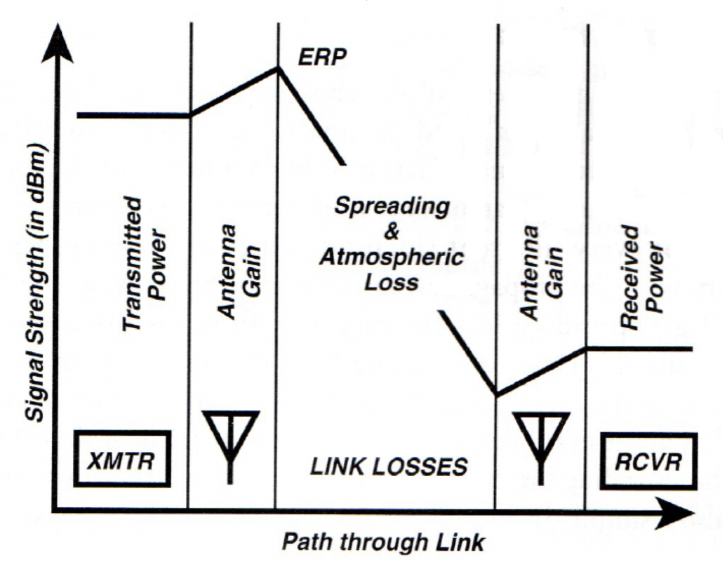
\includegraphics[scale=0.4]{images/1-signal-strength.png}
	\caption{Signal strength across the channel (ERP = Effective Radiated Power)}%
	\label{fig:signal-strength}
\end{figure}

\paragraph{Receiver sensitivity}
The weakest signal from which the receiver can still obtain the desired
information signal. Depends not just on the antenna gain, but also on other
factors such as the noise.

\paragraph{Decibel}
\begin{itemize}
	\item dBm --- signal strength in dB / 1 milliwatt mW
	\item dBW --- signal strength in dB / 1 watt W
	\item dBi --- antenna gain in dB / antenna gain of isotopic antenna in dB
\end{itemize}
Calculating a value in dB \[ dB(n) = 10 \log_{10} (n) \quad \text{ and } \quad dBm(n) = 10 \log_{10} (n / 1 mW) \]

\paragraph{Power Spectral Density diagram}
Depicts the power density (in dB) for a range of frequencies. In simple terms,
it shows how strong the signal is at a given frequency.

For a signal $x_T(t)$ defined between $(-\frac{T}{2}, \frac{T}{2})$, its power
in the time domain will be \[P = \lim_{T\rightarrow \infty} \frac{1}{T} \int |x_T(t)|^2 dt \] and its power in the frequency domain will be \[PSD(f) = \lim_{T\rightarrow \infty} \frac{1}{T} \int |X_T(f)|^2 df \]

\paragraph{Security Goals}
Reasons: \textit{security} (integrity, confidentiality, authentication),
\textit{regulatory} (personal liability for misuse of one's network access),
\textit{safety} (RF-enabled implants).

Just reducing transmission power, hoping that the attacker will be too far away
to listen on / send / modify messages, is NOT a solution. In fact, WiFi signals
can be received 10 km away, and similarly Bluetooth at 1 km distance (with
good, directed equipment).

Example: \textit{Passive Keyless Entry and Start systems (PKES)}, i.e.\
wireless car keys. Wrongly assume communication implies physical proximity
(relay attack). Needs: Authenticated proximity verification, message
authentication.

\subsection{Questions}
\textbf{Does a wireless channel, in general, affect all frequencies of a signal equally?} It depends on what kind of noise/interference is present on the channel. If it's general thermal noise, then yes, all frequencies will be generally affected in a similar way. However, if there are other communications happening, then the frequencies used by those transmissions will have a greater noise level.
Also, higher frequency signals suffer from greater attenuation due to the distance traveled compared to lower frequency signals.

\textbf{Which two properties of the wireless channel are leveraged by systems that rely on those for physical-layer based key establishment?} Channel impulse response and received signal strength.

\textbf{Describe the effect of increasing or decreasing the sub-carrier spacing in an OFDM modulated signal. Assuming the overall bandwidth of the channel stays the same, how does the sub-carrier spacing affect Symbol length, Throughput and complexity of the receiver?} TODO % TODO: increasing sub carrier spacing decreases symbol length because it increases symbol time ???
% TODO: A longer symbol length makes it more resilient against multi-path interference, but it probably needs a more complex receiver.
% TODO: Throughput should stay the same ????
\newpage

\section{Jamming Basics}

\paragraph{Jamming}
Entirely preventing or reducing the ability of communicating parties to pass information, either intentionally or unintentionally.

The jamming signal needs to have the same frequency as the modulated signal.
If the latter is unknown to the attacker, they thus need to jam a wide bandwidth of frequencies to be successful.

Effectively, jamming is always a power play.

\paragraph{Symbol}
Carries one or more bit of information, depending on the modulation scheme.

\paragraph{Symbol Jamming}
Corrupts symbols such that the receiver can EITHER no interpret them OR interprets them incorrectly.\\
Targeted, low-power jamming of specific symbols is hard!

\paragraph{Communication Jamming}
Corrupts enough bits that the information cannot be reconstructed any more, despite error correction.

\paragraph{Jamming-to-Signal Ratio J/S} = $J -  S$, i.e. the difference between the jamming signal and the modulated signal in dB.
A ratio $\geq 0$ usually results in successful jamming.

\paragraph{Burn-through range}
Range in which communication still succeeds, despite jamming.

\paragraph{Attacker model} \mbox{} \\
% taken from the following chapter/deck of slides
Types: responsive, sweep, random \\
Actions: jam, insert, modify (= overshadow) \\
Power to jam/insert/modify: $P_j, P_t, P_o$ \\
\# channels to jam/insert/modify: $c_j, c_t, c_o$ \\
Total strength/power $P_T$ \\
$$ c_j P_j + c_t P_t + c_o P_o \leq P_T$$

\subsection{Jamming Resistant Communication}

\paragraph{Basic principle}
If you cannot fight (i.e. have too little power), RUN, HIDE or WAIT.
And get ad advantage over the attacker: use a shared secret.

\paragraph{Frequency Hopping Spread Spectrum FHSS}
Regularly change transmission frequency.
The pseudorandom frequency sequence is derived from a shared secret.
Sender and receiver \textbf{must} be synchronised.

Note that frequency hoppers can be detected and located, simply by looking over time from which direction someone is sending on changing frequencies.

Possible attacks:
\begin{itemize}
	\item \textbf{Partial band jammer:}
	Distribute jamming power over a subset of all hopping frequencies to achieve $J/S=0$ at least on that range.
	\item \textbf{Follower jammer:}
	Detects on which frequency communication occurs and then jams it.
	Can be protected against by using error codes (since only the final bits will be corrupted).
\end{itemize}

\paragraph{Direct Sequence Spread Spectrum DSSS}
Spreads the baseband over a larger bandwidth using a shared secret (narrowband to broadband). \\
Since the transmission power remains the same, the power density at any given frequency decreases.
Thus the spread signal can effectively ``hide under the noise'' (\autoref{fig:dsss-psd}).

To spread over more frequencies, we need a higher symbol/bit rate.
To achieve this the information signal is multiplied with a high-frequency pseudorandom sequence called \textbf{chips} or \textbf{spreading code}.
The result resembles \textbf{white noise}.
See \autoref{fig:dsss}.

During de-spreading, the signal is again multiplied with the same spreading code.
De-spreading thus converts the wideband signal into a narrowband one (this works due to the autocorrelation properties of the spreading code).
At the same time, any narrowband interference is spread out.
\\
Thus DSSS is more robust against (un)intentional interference and multipath effects, and narrowband jamming requires much more power.
Broadband jamming is possible, but inherently requires much power.

Detecting DSSS signals is difficult, but not impossible (energy detection of strong signals, signal characteristics such as constant chip rate).
Interception and modification is hard.

Example usages: GPS, 802.11b WiFi, CDMA (used in 3G).
Non-military applications mainly use DSSS for interference-resistance and use public spreading codes.
They are thus still vulnerable to malicious jamming as DoS.

\begin{figure}
	\centering
	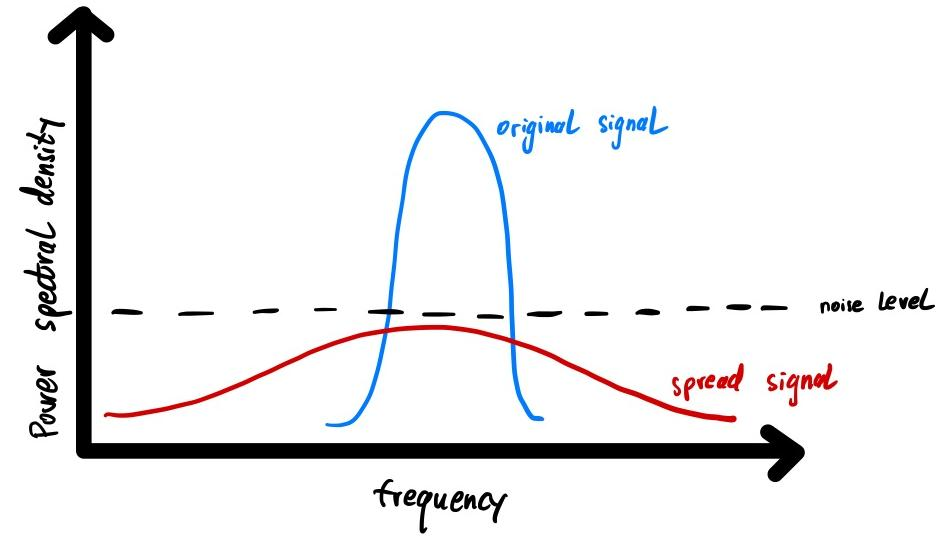
\includegraphics[scale=0.4]{images/2-dsss-psd.jpg}
	\caption{DSSS -- hiding under the noise}
	\label{fig:dsss-psd}
\end{figure}

\begin{figure}
	\centering
	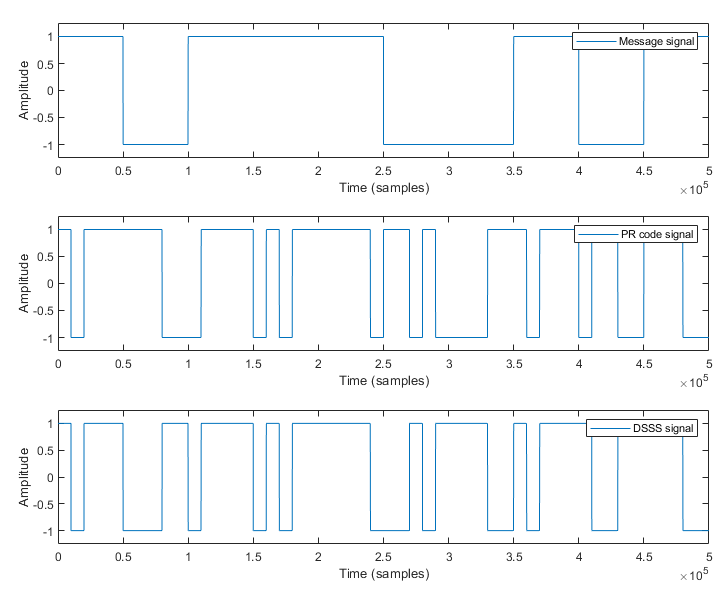
\includegraphics[scale=0.6]{images/2-dsss.png}
	\caption{DSSS -- baseband signal, spreading code, spread signal (top to bottom)}
	\label{fig:dsss}
\end{figure}

\paragraph{Processing Gain PG}
Ratio of the spread bandwidth to the baseband bandwidth, in dB.


\paragraph{Chirp Signal / Sweep Signal}
Signal in which the frequency increases and decreases over time (``sweeping'' over a bandwidth much wider than the baseband bandwidth).
Narrowband and partial-band jamming are prevented, follower jamming not so much

\paragraph{Code-Division Multiple Access CDMA}
Multiple transmitters sending in the same area simultaneously, but using different spreading codes.
Allows sharing of the same frequencies/bandwidth without interference.

\newpage

\section{Jamming-Resistant Broadcast}

\paragraph{Broadcast Communication}
One sender, many receivers. Inherently open: receivers may join and leave at any time. \underline{All} receivers listen (c.f.\ multicast). E.g.\ radio (FM/AM), GPS.\@

\paragraph{Challenges when securing broadcast}
many and unknown receivers, colluding receivers, internal + external attackers.
In particular, plain spreading techniques (with group keys) do not work --- an internal attacker can use their knowledge to jam other receivers.

\paragraph{Based on FHSS}
Broadcast Anti-Jamming System due to Desmedt et al. \\
Base station transmits on multiple frequencies simultaneously.
Each receiver listens on a subset of frequencies at a given time.
Protects against $j-1$ colluding receivers, ensuring that each receiver has at least one non-jammed channel.

\begin{itemize}
	\item \textbf{[Public] Channel Allocation Table:}
	Defines which channels any receiver should listen on, such that $j-1$ receivers do not cover all channels of any other receiver (set coverage).
	\item \textbf{[Secret] Frequency Allocation Table:}
	Mapping from channel id to frequencies.
	Derived using a PRG.
	The complete table is only known to the base station.
\end{itemize}

\underline{Disadvantages}:
effectively a multicast solution since it requires a shared secret between the base station and each receiver.

\paragraph{Based on DSSS}
Dynamic Jamming Mitigation due to Chiang and Hu.
Counteract jamming by using a balanced binary key tree.
\\
Each node in the tree corresponds to a spreading code $C_i$.
Each receiver $N_i$ is assigned a leaf and knows all codes on the path from the root to that leaf.
\\
The base station transmits on (a) a disjoint cover of codes (i.e. all users can decode exactly one code) and (b) a set of test codes.
If a client receives a test code but not the detectable code, it reports jamming.
\\
Splitting and reforming of the tree enables jamming mitigation.

\underline{Disadvantages}:
requires highly flexible, powerful base station.
Requires a feedback channel.
Requires a growing number of shared secrets (and receivers must be known).

\begin{figure}[h]
	\centering
	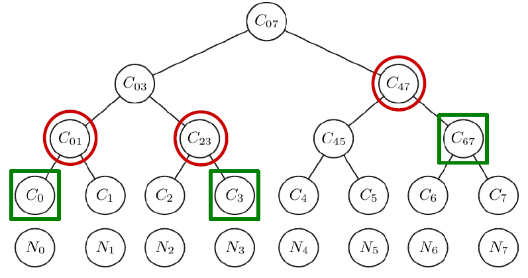
\includegraphics[scale=1.4]{images/3-chiang.png}
	\caption{Dynamic Jamming Mitigation -- cover codes (red circle), test code (green square)}
	\label{fig:chiang}
\end{figure}

\paragraph{Anti-Jamming---Key-Establishment Dependency}
Above techniques lead to a circular dependency.
We need techniques without shared secrets!
Idea: if we cannot coordinate sender and receiver, then don't even try.

\begin{figure}[h]
	\centering
	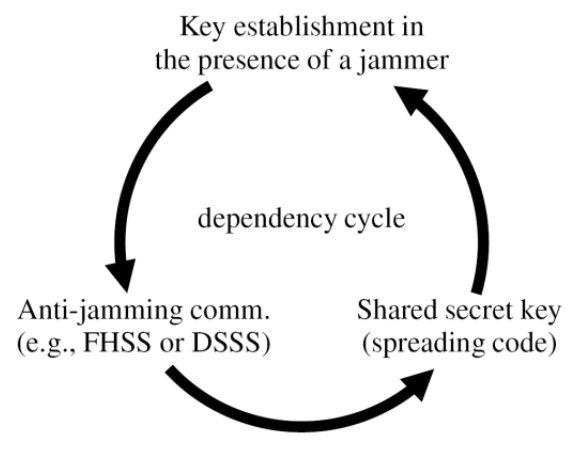
\includegraphics[scale=0.4]{images/3-jamming-key-cycle.png}
	\caption{Circular dependency between anti-jamming and key establishment}
	\label{fig:jamming-key-cycle}
\end{figure}

In addition, pre-loading shared keys is full of problems:
requires a trusted party, key revocation, new clients joining, etc.

\paragraph{Uncoordinated Frequency Hopping Spread Spectrum UFHSS}
Neither attacker nor legitimate receivers can predict which channels are used.
Equivalent to FH in terms of jamming protection (but not in throughput).

Transmitter steps:
\begin{enumerate}
	\item Fragment message
	\item Link fragments (against insertion)
	\item Encode packets (ECC against jamming)
	\item Repeated transmission while hopping on frequencies
\end{enumerate}

Receiver steps: same process but reversed (plus packet ordering).
Hops from one frequency to the other (sequentially is fine), in the hope of receiving a fragment.

\begin{figure}[h]
	\centering
	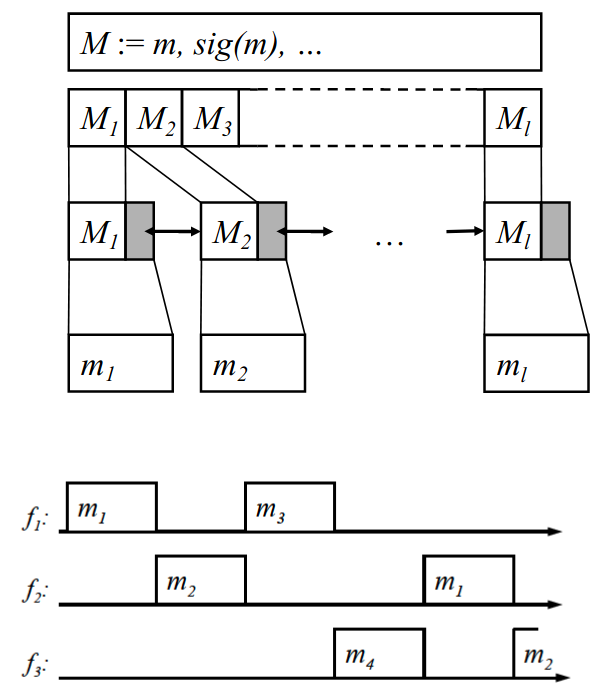
\includegraphics[scale=0.4]{images/3-ufh.png}
	\caption{UFH transmitter steps}
	\label{fig:ufh}
\end{figure}

\underline{Issue with fragment linking:} \\
The signature is only verified at the end for the entire message.%
\footnote{The signature is based on public-keys and a mutually trusted -- but potentially offline -- certificate authority CA.}
Since there are exponentially many combinations for re-assembly, the attacker can now perform a DoS on a logical (rather than physical) level (pollution attack).
\\
Solution: cryptographic linking of fragments (but without a shared key).
E.g. hash linking, one-way accumulators, short signatures.

\underline{Disadvantages}:
Throughput up to 1000x less than Frequency Hopping.
Higher latency (depending on attacker strengths, i.e. how high the chances are that the receiver gets a packet).

\begin{figure}[h]
	\centering
	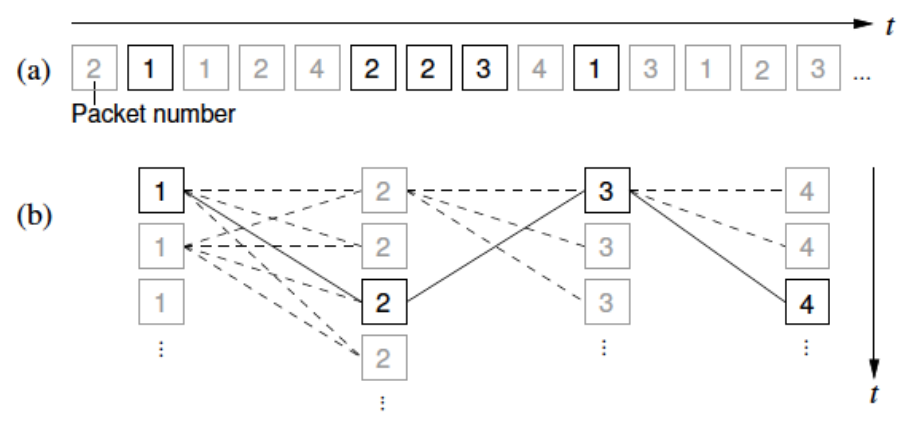
\includegraphics[scale=0.4]{images/3-ufh-fragment-linking.png}
	\caption{UFH fragment linking -- exponentially many candidate messages}
	\label{fig:ufh-fragment-linking}
\end{figure}

\paragraph{Uncoordinates Direct Sequence Spread Spectrum UDSSS}
Neither attacker nor legitimate receivers can predict which spreading codes are used.
The public code set $C$ is composed of $n$ code sequences, each containing $l$ spreading codes.%
\footnote{This allows a message to be fragmented into $l$ pieces.}
Despreading is done by trial-and-error: it requires the correct code sequence and correct synchronisation (which fragment are we at?).
The message is also repeatedly sent because of possible jamming -- possibly in parallel to improve throughput.

\underline{Optimisation}: first transmit the message $M$ with a secret spreading code $K$ using DSSS.
Then transmit the spreading code $K$ using UDSSS.
\\
Advantage: quicker decoding, longer messages, flexible security level.



\newpage

\section{Security of Global Navigation Satellite Systems GNSS}

\paragraph{Overview}
Orbiting satellites transmit their location and a precise timestamp.
Receivers collect these navigation messages and their arrival time and use \textbf{triangulation} to calculate their own position.
Satellites are positioned such that at least four are always in sight on any point on Earth.

Three segments: users, satellites, ground control.%
\footnote{There are of course issues with special and general relativity that mess with the time.}

\paragraph{Signalling}
Each satellite modulates the navigation message with a spreading code (coarse acquisition C/A for civilians (public), precision P/Y for military (secret)).
The spread signal is then modulated onto a carrier.
\\
Individual satellites use individual spreading codes to allow distinction.
\\
GPS sends on two carrier frequencies at the same time, L1 (1575.42 MHz = 10.23 MHz $\times$ 154) and L2 (1227.60 MHz = 10.23 MHz $\times$ 120).%
\footnote{This only applies to military. The civilian C/A is only transmitted on L1.}
Apart from jamming resistance and redundancy, this also allows to calculate the ionospheric delay error.
\\
Due to atmospheric attenuation, down on Earth the GPS signal is well below the thermal noise.

\paragraph{Navigation message}
Each message consists of 25 frames.
Each takes 30 sec to transmit, so the total time is 12.5 min.
\\
Each frame contains: satellite clock + health data, 2x ephemeris (orbit details), other data + almanac (orbital + clock details).

\paragraph{Time of Arrival TOA}
Travel time of the signal from the satellite to the receiver.
Used to calculate the distance and thus eventually the receiver position.
Found by sliding the spreading code over the received message until a correlation peak.

\paragraph{Spoofing attacks}
Messages are unauthenticated (for practical reasons, else they would become too long).
\\
By sending stronger signals, overshadowing the legitimate ones, an attacker can modify the \textit{navigation message contents} (transmission time, satellite location) or their \textit{time of arrival} (retransmitting captured signals with a temporal shift), resulting in a wrong location being calculated.
\\
This is an issue in civilian GPS (messages can be generated and delayed) as well as in military GPS (messages can only be delayed since they are encrypted).
Unfortunately, commercial GPS signal generators are becoming increasingly cheap.


\subsection{Spoofing Detection and Mitigation}\label{sec:gps-spoof}

\paragraph{Types of countermeasures}
\begin{itemize}
	\item \textbf{Infrastructure/protocol:} e.g. cryptographic authentication of navigation messages
	\item \textbf{Receivers:}
	Use physical-layer characteristics of the signal to validate the signal as well as the calculated position/velocity/time.
	E.g. direction of arrival, carrier phase, signal strength, etc.
\end{itemize}

\paragraph{Angle of Arrival AoA}
Use multiple antennas (e.g. on both ends of a ship) to calculate the angle of arrival through the phase difference and the known distance between the antennas (see beam steering, \autoref{fig:beam-steering}).
In a spoofed scenario, the angles would all be very similar.
Restricts the locations from which the attacker can successfully spoof.

\underline{Problems:}
Attacker can use drones to spoof signal from more realistic angle.
Reflection of legitimate signal of buildings (thus reaching the receiver at a shallower angle) could be wrongly classified as spoofing.
Computationally expensive phase measurement.
Hardware modification.

\paragraph{Monitor Signal Characteristic Changes}
Over time, monitor signal properties such as AGC (Automatic Gain Control), noise level, number of satellites, spatial diversity (AoA) or the autocorrelation peak.
Abrupt changes in any of these indicate presence of spoofing.

\paragraph{Seamless takeover attack}
The attacker starts transmitting a copy of a legitimate GPS signal in sync with the original one, but at low power, having no influence on the receiver.
Then the attacker slowly starts increasing the power, until the receiver prefers the attacker signal.
Now the attacker can change the GPS signal, and the receiver will keep following. 

\begin{figure}
	\centering
	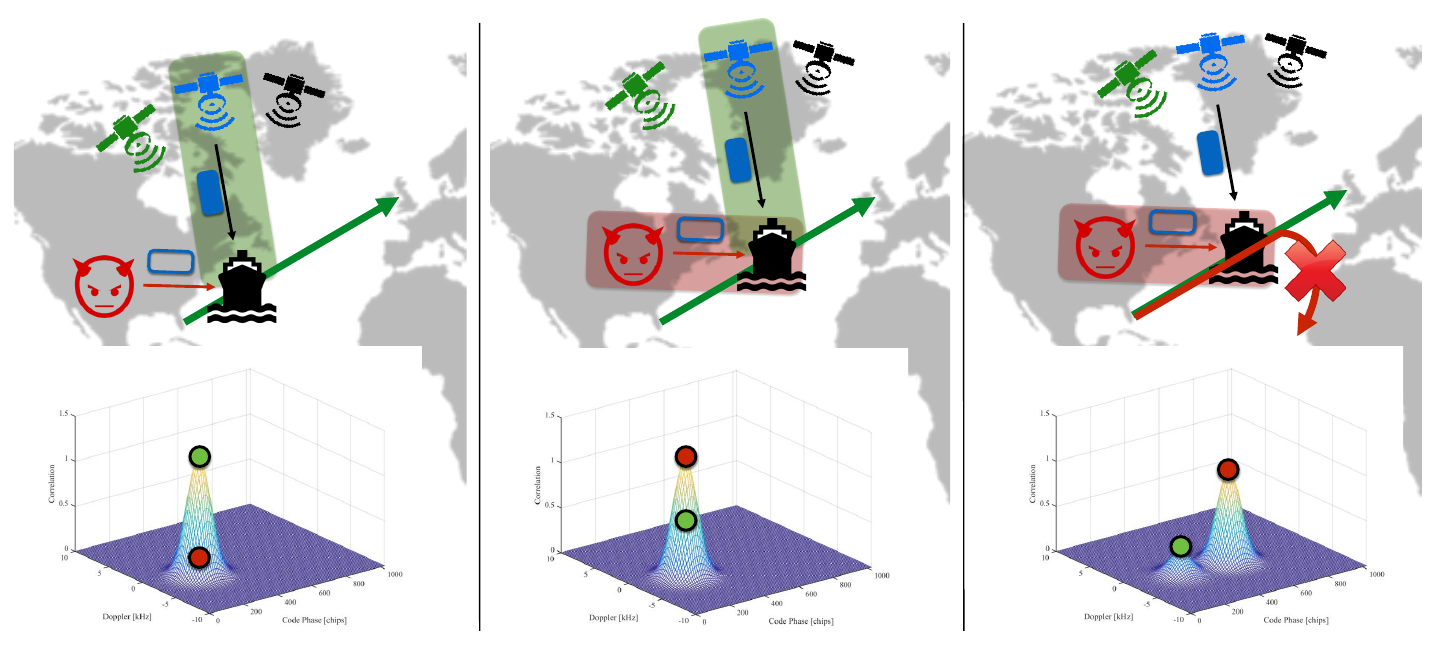
\includegraphics[scale=0.4]{images/4-seamless-takeover.png}
	\caption{Seamless takeover attack}
	\label{fig:seamless-takeover}
\end{figure}

\paragraph{SPoofing REsistance GPS rEceiver SPREE}
Leverage peak tracking (of \underline{all} signal peaks) to detect seamless takeover attacks.
Navigation message inspection detects content spoofing.

\paragraph{Cryptographic approach (Kuhn)}
\begin{enumerate}
	\item At time $t$: satellite uses secret spreading code.
	Receiver uses a broadband receiver to capture the entire band.
	\item At time $t+dt$: Satellite disclosed code, signing the disclosure with its secret key.
	Receiver verifies signature, de-spreads the signal.
\end{enumerate}

\underline{Advantages:}
Prevents fake signal generation and individual signal delay.

\underline{Disadvantages:}
Requires pre-shared public satellite keys.
Slightly inefficient (longer latency until signal lock).
Requires loose synchronisation (after $dt$ the attacker knows the spreading code and can spoof).
Does NOT prevent full-band delay.
Relay/replay attacks (record signal and replay full band in another location in real time).


\newpage

\section{Secure Ranging}

Secure Ranging, or distance measurement, is commonly used, for example, in wireless car keys, contact tracing in a pandemic, payments, automation.

\textbf{Replay attacks} are an issue, allowing an attacker to \hl{make devices appear physically closer} (e.g.\ if the device naively use the observed signal strength to derive the distance).
\\
\underline{Goals:}
(Provably) secure ranging, protecting against all logical and physical attacks and all attacker abilities, with a \hl{focus on preventing distance reduction}, that should bind distance to identity.

\paragraph{Current techniques (overview)} \mbox{} \\
Non-Time-of-Flight:
\begin{itemize}
	\item Received Signal Strength Indication [RSSI] (WiFi, Bluetooth, 802.15.4, NFC, RFID) --- \textit{insecure}
	\item (Multi-carrier) phase measurement\footnote{The distance is proportional to the phase.}
	      --- \textit{insecure}
	\item Frequency-Modulated Continuous-Wave FMCW --- \textit{insecure}
\end{itemize}

Time-of-Flight:%
\footnote{
	Calculate via $d = c \cdot (t_{tof} - t_{proc}) / 2$
	where $t_{tof}$ is the time between sending and receiving the signal and $t_{proc}$ is the known processing time on the responding device. \\
	In general, manipulating time is harder than manipulating signal properties (strength, phase).}
\begin{itemize}
	\item Chirp Spread Spectrum (802.15.4 CSS) --- \textit{insecure}
	\item Ultra Wide Band UWB (802.15.4z) --- \hl{\textit{proposed}}
	\item WiFi 802.11az, 5G --- \textit{first efforts to secure OFDM-based}
\end{itemize}

\paragraph{Model}
On a logical level, we have a \textbf{verifier V} and a \textbf{prover P}, between which we want to measure the distance.
A \textbf{malicious party M} attacks this.

% See also the \href{https://www.iacr.org/workshops/fse2013/slides/Slides02.pdf}{Brands-Chaum protocol} (not discussed in HS20).

Additionally, we assume the worst case for the users but the best case for the attacker (bad channel/noise/multipath versus perfect channel $\rightarrow$ attacker guesses will look like noise).

\begin{figure}[h]
	\centering
	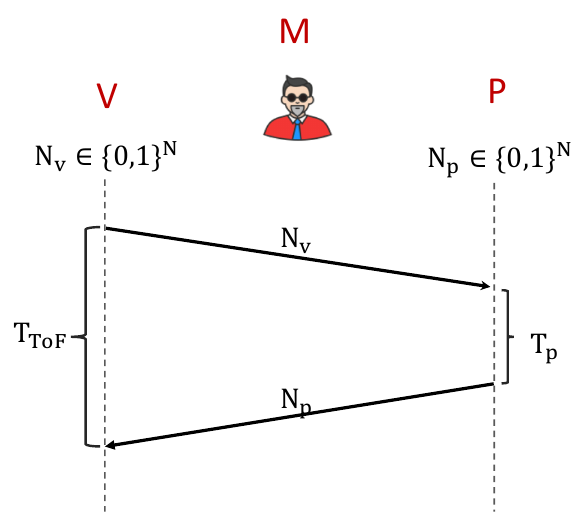
\includegraphics[scale=0.4]{images/5-model.png}
	\caption{Model of the distance bounding scenario}%
	\label{fig:ranging-model}
\end{figure}

\paragraph{Types of attacks (frauds)}
\begin{itemize}
	\item \textbf{Distance fraud:} A dishonest $P$ tries to change its distance to $V$.
	\item \textbf{Mafia fraud:} Honest $V, P$ being attacked by an external $M$.
	\item \textbf{Terrorist fraud:} Dishonest $P$ and $M$ collude to change $P$'s distance.
	\item \textbf{Distance hijacking:} Dishonest $P$ leverages an honest $P$ to change its distance.
\end{itemize}


\paragraph{Logical Layer}
Distance reduction prevented using challenge-response protocols with time measurements (i.e., distance-bounding). V and P share a secret key unknown to M. V and P exchange messages that are (in part) unpredictable to M. STS cannot be predicted by M (before it is sent).

\begin{figure}[h]
	\centering
	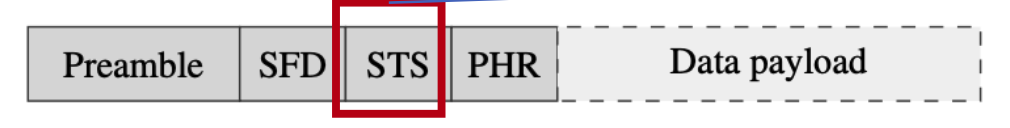
\includegraphics[scale=0.8]{images/5-sts.png}
	\caption{Scrambled Timestamp Sequence}%
	\label{fig:sts}
\end{figure}

\paragraph{Distance Commitment}
Distance commitment is the Time of Arrival measured over a public preamble and then verified using payload pulses generated using UWB pulse reordering. The timing of the preamble is binding. An attacker needs to advance payload if he advances the preamble. It's the way of knowing the distance between transmitter and receiver.
As the attacker needs to advance the payload as well, he needs to guess and send before the legitimate pulse arrives, which gives him immediate feedback, and the attacker can then adjust the subsequent pulses in order to reach the needed net energy level.


\paragraph{Distance Bounding}
A prover who wants to prove its position should quickly receive $N_V$, compute $Ff(N_V,N_P)$ and send it.
The verifier estimates prover's processing time $=t_p$. \hl{If the attacker's processing time is $0$, then he can cheat by $t_p/2$}. Thus, ideally, $t_p=0s$; usually, though, $t_p=1-2ns$ which means that the attacker can only shorten the distance by $15-30cm$.
\begin{figure}[h]
	\centering
	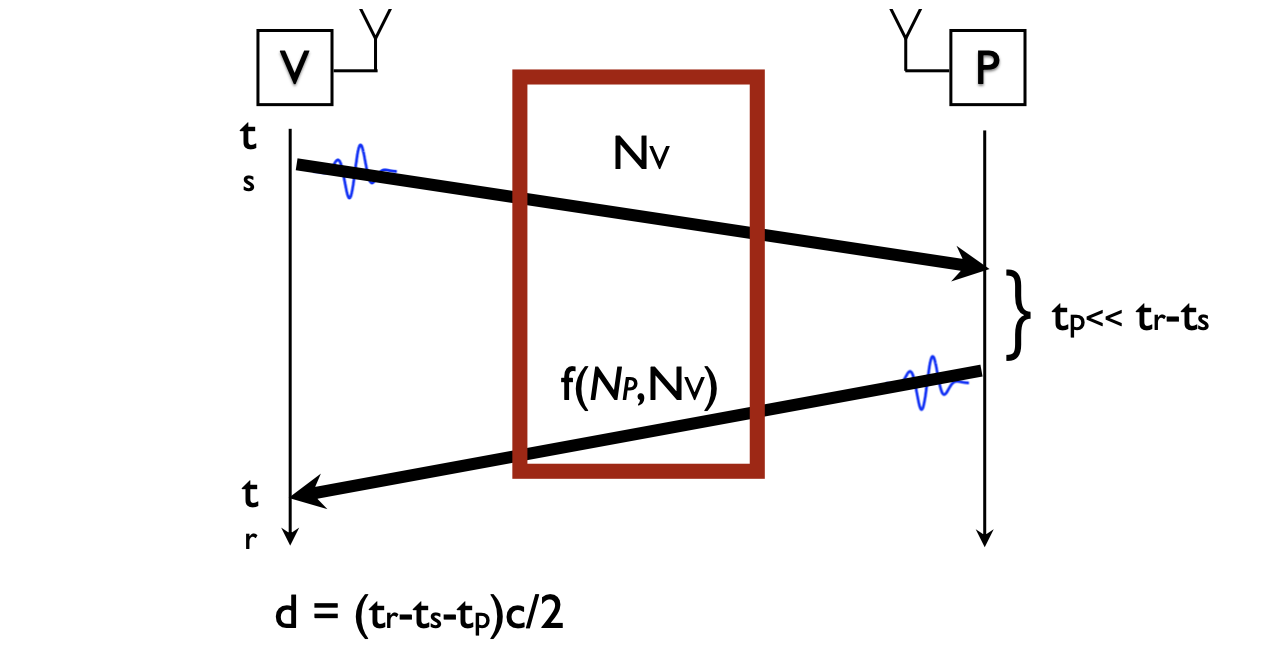
\includegraphics[scale=0.4]{images/5-dist-bounding.png}
	\caption{Distance Bounding}%
	\label{fig:dist_bounding}
\end{figure}
An evolution of this is Challenge reflection with Channel Selection, where the prover only needs to reflect $N_V$ and the verifier does all the work. This reduces $t_p$ to $0$.

\paragraph{Physical Layer: Representing bits as pulses (UWB)}
There are two design options to represent a bit: either with a \textbf{single strong pulse} or a \textbf{sequence of weaker pulses}.
Single pulses may not be detected reliably (distance, interference), so the aggregate over several pulses is the preferred representation.

\begin{figure}[h]
	\centering
	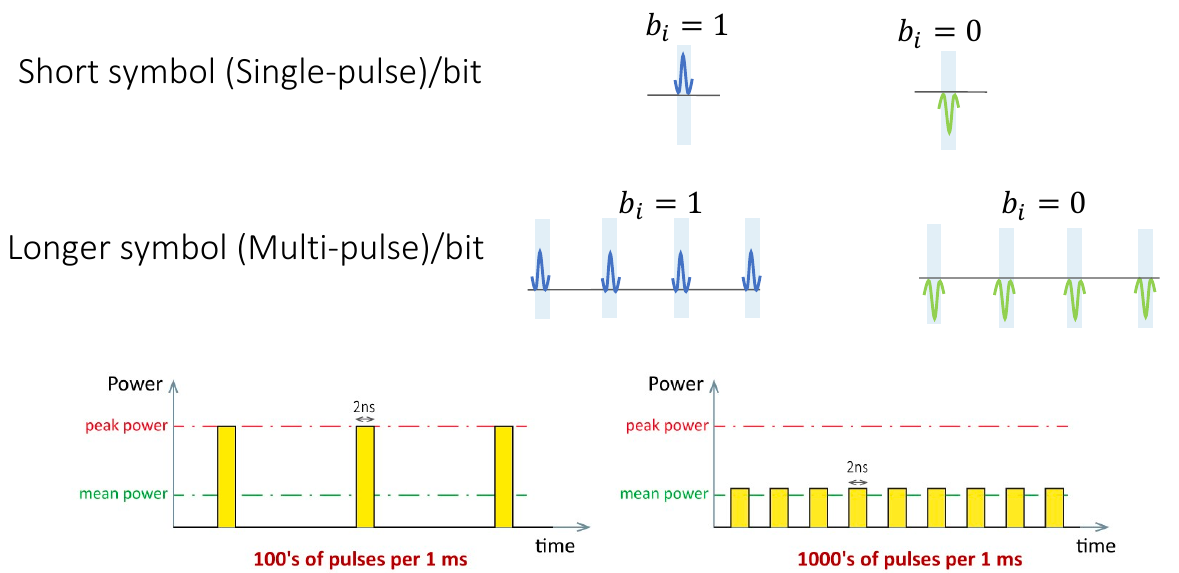
\includegraphics[scale=0.3]{images/5-single-multi-pulse.png}
	\caption{Bit representation: single- versus multi-pulse}%
	\label{fig:single-multi-pulse}
\end{figure}


\subsection{Early-Detect/Late-Commit attack (ED/LC)}
This attacks shortens the distance, since the receiver receives the first symbols earlier than it should have.

\begin{enumerate}
	\item Attacker sends noise (at time $T_A$)
	\item Attacker learns correct symbol (at time $T_{ed}$)
	\item Attacker commits to correct symbol (at time $T_{lc}$), by sending the remaining pulses such that the sum over all pulses matches.
\end{enumerate}

Note that this attack is not possible with single pulses.
A single pulse is usually $1-2$ ns long, so the attacker can cheat by at most $15-30$ cm (performance/security tradeoff).

\begin{figure}[h]
	\centering
	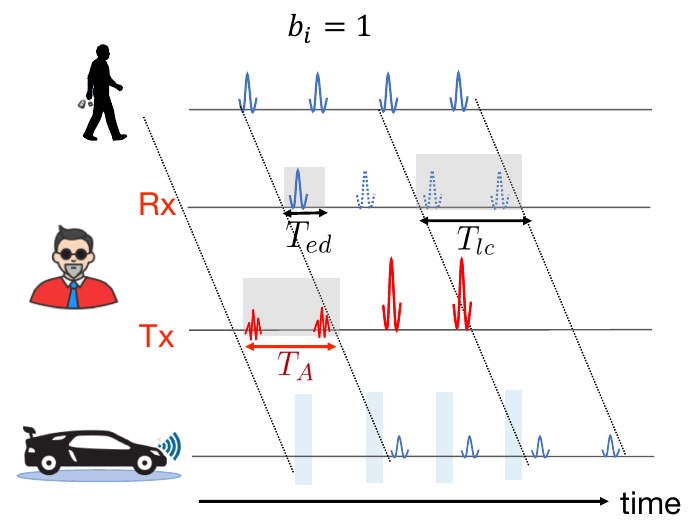
\includegraphics[scale=0.3]{images/5-edlc.png}
	\caption{Early-Detect/Late-Commit attack (ED/LC)}%
	\label{fig:edlc}
\end{figure}

\paragraph{ED/LC Solution 1: Pulse Reordering UWB-PR}
Interleave pulses of subsequent symbols according to some cryptographic reordering.
Thus the start and end time of a symbol is unpredictable, and the attacker can only guess.
\\
The probability of an attack's success decreases with the increase of the number of reordered bits.

\begin{figure}[h]
	\centering
	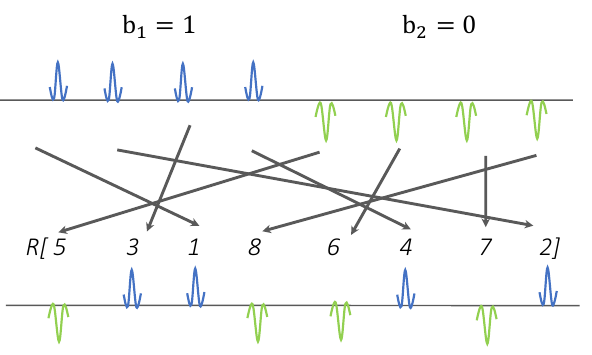
\includegraphics[scale=0.45]{images/5-pulse-reordering.png}
	\caption{Pulse Reordering}%
	\label{fig:pulse-reordering}
\end{figure}

\paragraph{ED/LC Solution 2: Variance Based Detection}
Statistically analyze the received versus the expected pulses.
This forces the attacker to ``guess better'' to reduce the variance and make their error indistinguishable from the noise.

\begin{figure}[h]
	\centering
	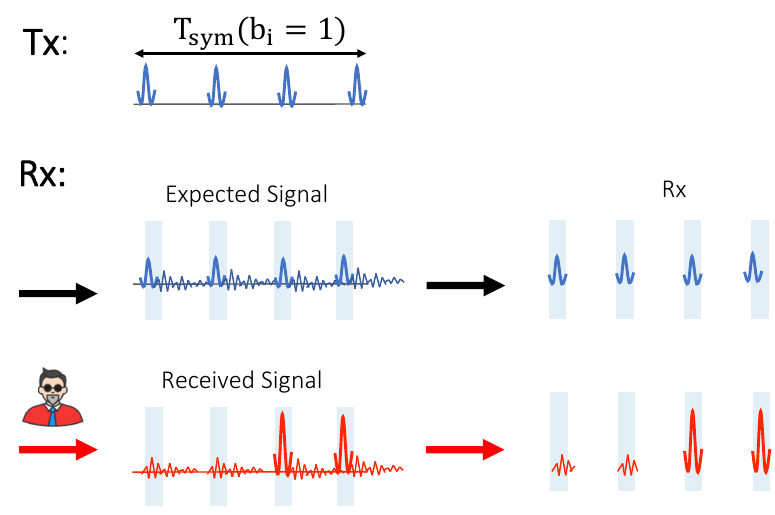
\includegraphics[scale=0.4]{images/5-variance-based.png}
	\caption{Variance Based Detection}%
	\label{fig:variance-based}
\end{figure}

\paragraph{ED/LC Solution 3: Scrambled Timestamp Sequence}

After the preamble (high correlation) which is used for ToF \textit{estimation},
send a Scrambled Timestamp Sequence STS (encrypted with a shared secret, low autocorrelation) to use for ToF \textit{verification}.
\\
See IEEE 802.15.4z.
Security not formally proven and unclear!

\begin{figure}[h]
	\centering
	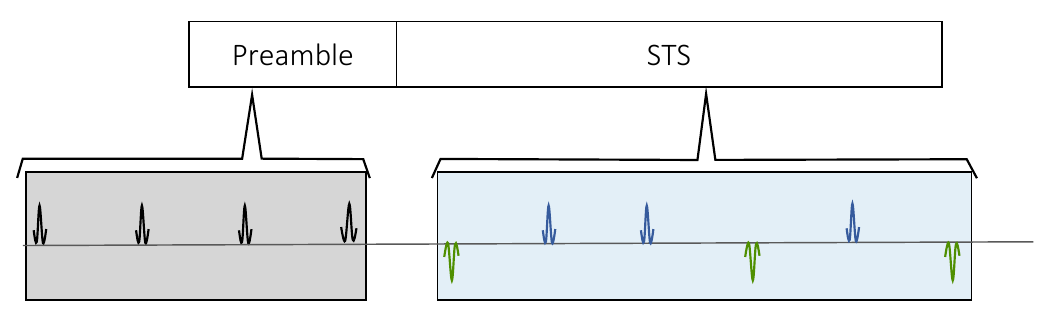
\includegraphics[scale=0.35]{images/5-scrambled-timestamp.png}
	\caption{Scrambled Timestamp Sequence}%
	\label{fig:scrambled-timestamp}
\end{figure}

\subsection{IEEE 802.15.4z LRP versus HRP}
\begin{table}[h]
	\centering
	\begin{tabular}{ll}
		\hline
		Low Rate Pulse LRP                & High Rate Pulse HRP                      \\ \hline
		Can use single pulse              & No single pulse (energy too low)         \\
		Multi-pulse with UWB-PR efficient & UWB-PR + variance-based seem inefficient \\
		Open  and simple security specs   & No open security analysis                \\
		Low-cost, low-energy              & More transparency needed                 \\ \hline
	\end{tabular}
\end{table}


In HRP, receivers cannot decode individual pulses. Instead, they first need to find the maximum autocorrelation peak (which is not the correct ToA) and then look for the Early Path (leading edge/correct ToA)
\begin{figure}[h]
	\centering
	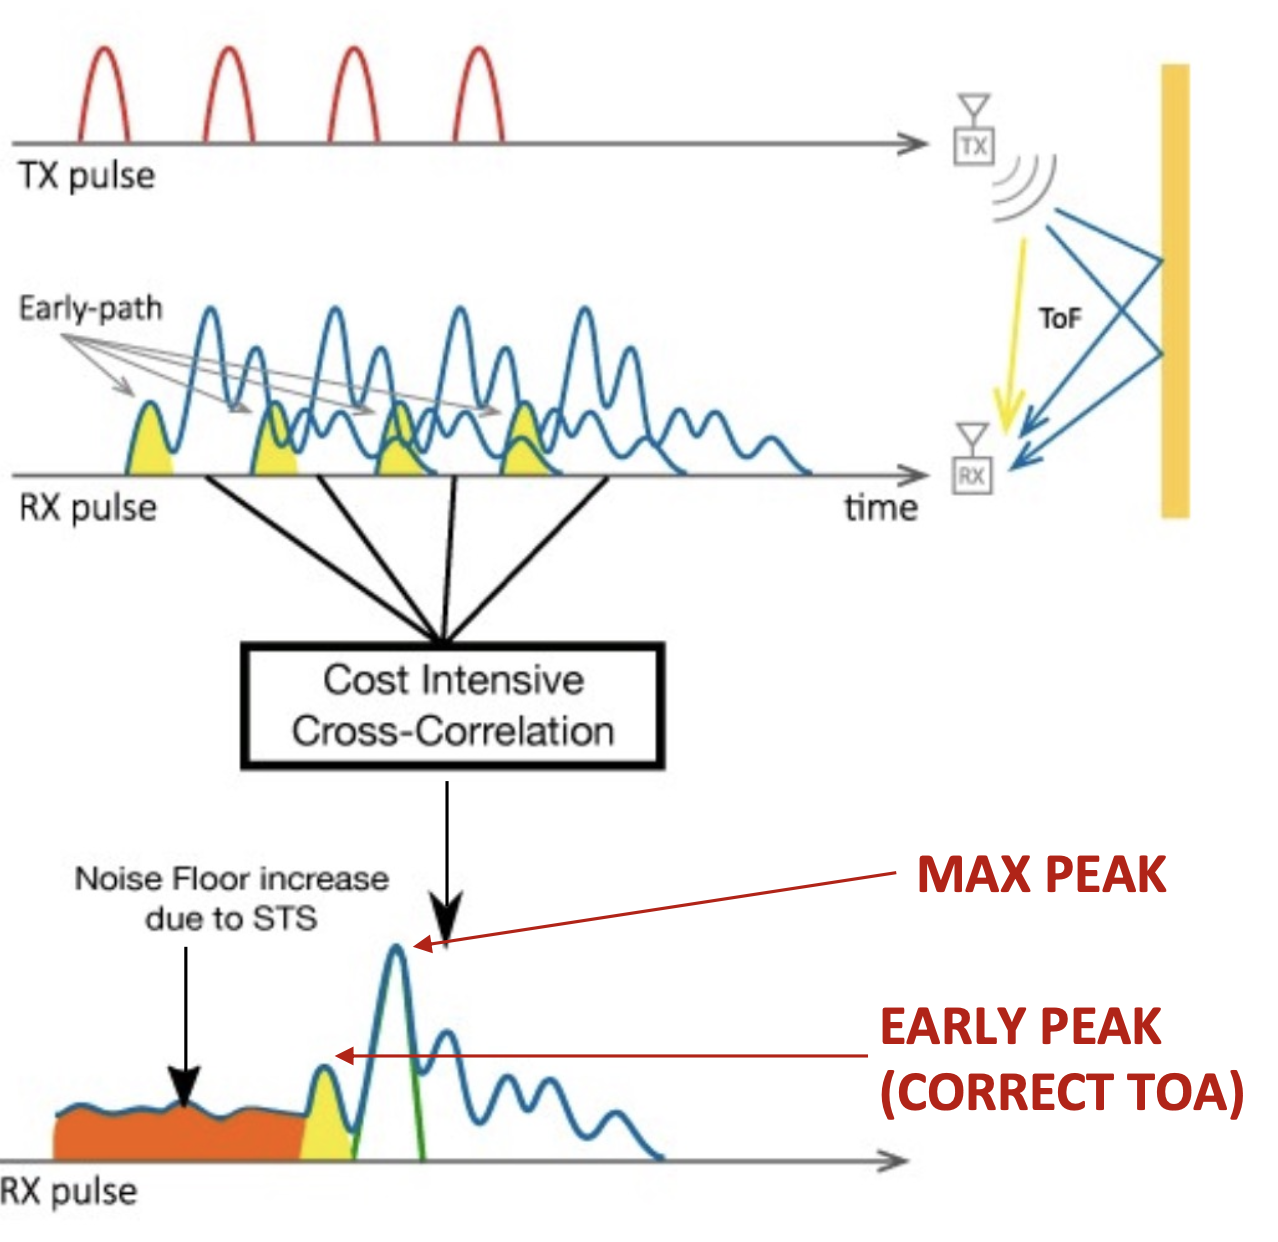
\includegraphics[scale=0.3]{images/5-early-peak.png}
	\caption{Early Peak}%
	\label{fig:earlypeak}
\end{figure}

\subsection{Ghost-Peak Attack}
This attack shows that physical-layer attacks on HRP are a real threat. Apple/NXP/Qorvo use hidden ToA estimation algorithms making it hard to evaluate if their HRP ranging systems are truly secure. Instead, these algorithms should be public and comprehensively evaluated.
Like with ciphers/signatures/MACs, their security should rely only on the unpredictability of the STS, not on the secrecy of the algorithms.
It resulted in a successful reduction of the perceived distance of $4-12$ meters.

\begin{figure}[h]
	\centering
	
\includegraphics[scale=0.45]{images/5-ghost-peak.png}
	\caption{Ghost Peak Attack}%
	\label{fig:ghostpeak}
\end{figure}

\paragraph{Main idea}
The attack basically consists in injecting a packet in-sync (micro-seconds) with the legitimate transmission but with varying power of Preamble, SFD, STS.\@ The attack is based on the assumptions that there is no knowledge of the keys shared between victim devices and the attacker is not able to predict the Scrambled Timing Sequence (STS).
The necessary equipment is inexpensive and easily purchasable.

\paragraph{Message Time of Arrival Code MTAC}
New class of cryptographic primitives that verify the integrity of message arrival time.
E.g.\ single-pulse, UWB-PR, Variance-based detection.

\begin{figure}[h]
	\centering
	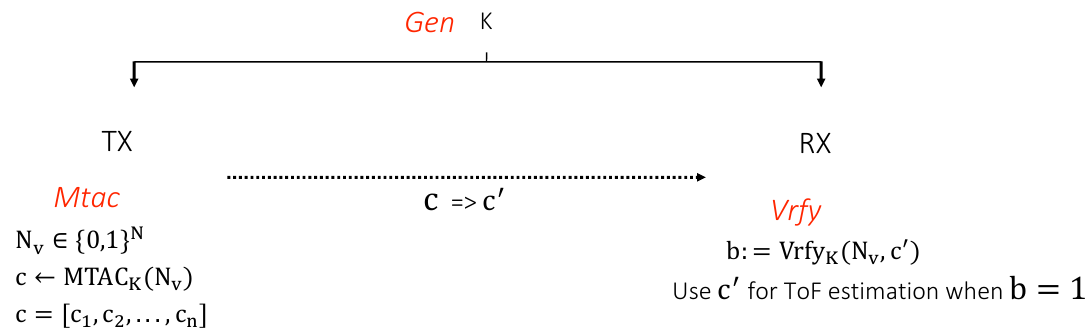
\includegraphics[scale=0.3]{images/5-mtac.png}
	\caption{Message Time of Arrival Code MTAC}%
	\label{fig:mtac}
\end{figure}

\paragraph{Verifiable Multilateration}
Multiple verifiers with known locations want to determine the position of a prover.
C.f. GPS trilateration.
E.g.\ to position autonomous cars using cell towers.


\paragraph{Future Work}
\begin{itemize}
	\item Secure Positioning (e.g.\ verifiable multilateration)
	\item WiFi 802.11 and 5G ranging (some initial work)
	\item Efficient implementation + deployment
\end{itemize}

\newpage

\section{Security in Critical Transport Infrastructures}


\paragraph{Air Traffic Control ATC}
\begin{itemize}
	\item \textbf{Primary Surveillance Radar PSR}:
	ground based, measures time delta between transmission and reflection $\Rightarrow$ independent.
	\item \textbf{Secondary Surveillance Radar SSR}:
	Transponder based interrogation $\Rightarrow$ dependent. \\
	Mode A (identification code), Mode C (identification code + barometric altitude), Mode S (selective addressing to interrogate a specific aircraft, used in \textit{Traffic Alert and Collision Avoidance System})
	\item \textbf{Automatic Dependent Surveillance-Broadcast ADS-B}:
	Aircraft determines its position via satellite and regularly broadcasts the result.
	Replaces functions of SSR, and enables inter-aircraft situational awareness.
\end{itemize}

\paragraph{Problem Statement}
Huge number of systems and protocols in aviation (see \autoref{fig:air-systems}).
None has confidentiality, integrity or authentication.
On the other hand, attacker capabilities grow as domain knowledge spreads and software defined radios become cheaper.
\\
At the same time change is incredibly slow due to certifications and legacy compatibility.

\begin{figure}[h]
	\centering
	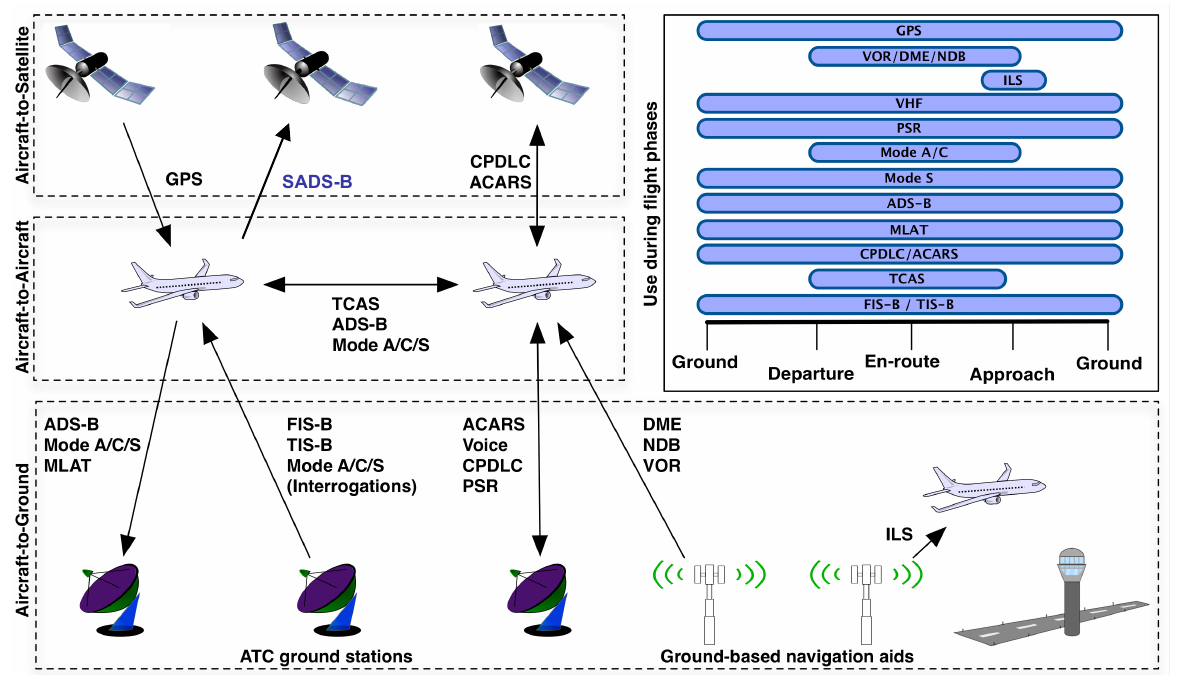
\includegraphics[scale=0.5]{images/6-air-systems.png}
	\caption{Overview of aviation systems}
	\label{fig:air-systems}
\end{figure}



\subsection{Privacy Issues in Aviation}

\paragraph{No confidentiality of aircraft-ground communication}
Clear-text transmission of passenger medical status, forgotten belongings, credit card transaction details, etc.

\paragraph{Proprietary crypto}
ACARS\footnote{Aircraft Communications Addressing and Reporting System}
datalink encryption uses a mono-alphabetic substitution cipher with a limited keyset hardcoded in a lot of private/military/government jets.

\paragraph{Aircraft identifiers}
Aircraft transponders have unique IDs that include aircraft type and operator.
These are not easily and legally changed (unless aircraft is sold).

\paragraph{No location privacy}
Aircraft are globally trackable by anyone.
Either using websites like Flight-Radar24 (heavily filtered), ADS-B Exchange, OpenSky Network.
Or collecting own data from SSR and ADS-B signals using a cheap radio.

\underline{Possible ``uses'' for tracking}:
government aircraft movement, mergers \& acquisitions (M\&A) activities.

\underline{Mitigations:}
Block aircrafts on tracking websites, obscure ownership (register to shell/trust companies), disable position broadcasts (still easily localised near departure/destination airports), use commercial transport.

\subsection{Security Issues in Aviation}

\paragraph{Attacks}
The usual candidates: jamming, modification, injection (ghost aircraft = DoS on ATC).

\paragraph{Safety vs Security}
\textit{Safety} is about dealing with accidents and failures.
We tackle it with experience (root cause analysis) and redundancy (decreasing the likelihood of failure of the entire system).

\textit{Security} on the other hand is concerned with protecting against an intelligent, adaptive attacker.
See the Swiss Cheese model in \autoref{fig:swiss-cheese}.

\begin{figure}[h]
	\centering
	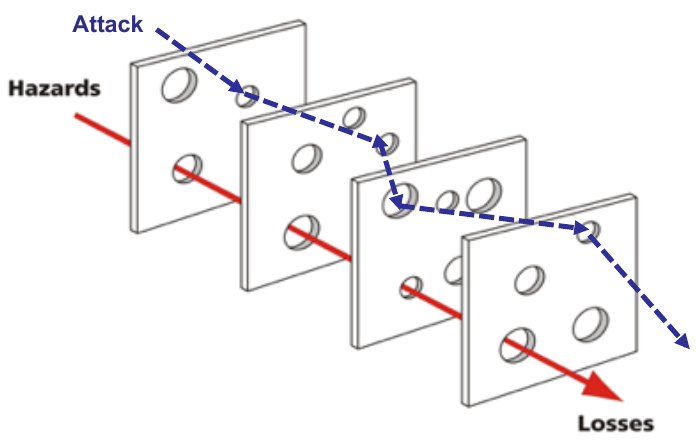
\includegraphics[scale=0.5]{images/6-swiss-cheese.png}
	\caption{Swiss Cheese Model: Safety vs Security}
	\label{fig:swiss-cheese}
\end{figure}

\paragraph{Traffic Collision Avoidance System TCAS}
Aircraft continuously predict each others' paths.
If the paths are too close but not yet at risk, a \textit{traffic advisory TA} is issued (and announced in the cockpit).
If they remain on a close path, a \textit{resolution advisory RA} is announced as compulsory instructions.

\underline{Attack:}
Attacker listens to target aircraft and injects TCAS responses, forcing a TA and RA, thus forcing the aircraft to make unwanted course changes (plus push pilots to reduce TCAS sensitivity).



\subsection{Short-term Security Countermeasures}

\paragraph{Cyber-Physical Countermeasures}
There won't be any real crypto any time soon.
In the meantime, exploit physical layer data (timing, signal strength, Doppler shift, etc) to validate signals.
Throw in some machine learning as well (for anomaly detection).
\\
This hopefully lifts the bar back up to nation-state-attackers-only,

\paragraph{Multilateration}
Use multiple ground stations to receive (and validate) signals from aircraft.

\paragraph{OpenSky Network}
Crowdsources ATC.
Volunteers install software-defined radios around the world to capture signals and publish them.

Short-term solution: rather than cryptographically authenticating messages between aircraft, use ground network to check if everybody else also received the same signal.

\underline{Advantages:}
Does not touch legacy systems, low cost, global coverage, flexible.



\subsection{Satellite and Maritime Infrastructures}

\paragraph{Satellite links}
Signals are receptable in a large area (continent-scale).
This allows tracking of e.g. military aircraft from far away.

\paragraph{Maritime VSAT} (Very Small Aperture Terminal). Still large and expensive.
Connects ships to IP network on land (WiFi, fleet monitoring, weather, navigation, cargo, etc).
Composed of a satellite uplink (large beam, since satellite needs to cover a large area $\Rightarrow$ can be captured from far away) and a directed downlink (towards a ground/land station).
\\
Example: \textit{Electronic Chart Display and Information System ECDIS} (paper chart/map replacement) receives updates via VSAT.

\underline{Analysis:}
Lots of interesting yet unencrypted traffic -- from standard DNS/VoIP/IMAP to specific ``ship data''.

\paragraph{TLDR} It's bad.


\newpage

\section{Physical Layer-based Security}


\subsection{Channel-based Key Establishment}

\paragraph{Unique channels}
In a complex, multi-path rich environment channel exhibit time-varying, stochastic and reciprocal fading.
For receivers separated by $> \lambda / 2$ their channels are \underline{not} correlated.

Thus the channels between sender $S$ and receiver $R$ are ``random'' and cannot be known/predicted by the attacker.
In particular, the attacker cannot remotely measure multipath fading components of the signal strength.

\paragraph{Key Agreement through Channel Properties}
We can leverage different properties of the channel, e.g. RSSI\footnote{Received Signal Strength Indication}, CIR\footnote{Carrier-to-interference ratio} or signal phase.

The generic steps are the following:
\begin{enumerate}
	\item Signal Acquisition and Quantisation
	\item Reconciliation (error correction, privacy amplification)
	\item Key confirmation
\end{enumerate}

\begin{figure}
	\centering
	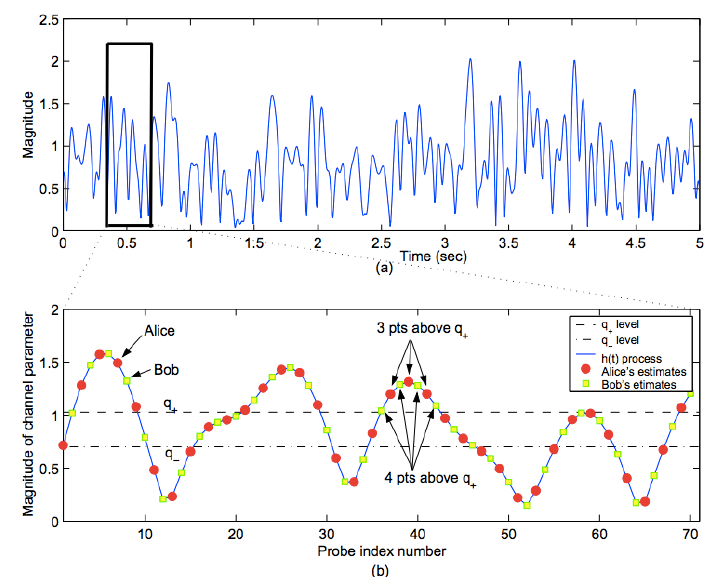
\includegraphics[scale=0.5]{images/7-channel-property.png}
	\caption{Measuring Channel Property Magnitudes over Time}
	\label{fig:channel-property}
\end{figure}

\paragraph{Analysis}
There are several disadvantages to this scheme:
\begin{itemize}
	\item No authentication: we establish a secret key, but with whom?
	\item No guarantees on the environment:
	Multi-path rich? Cannot be pre-measured? Receivers (and attacker!) at least $> \lambda / 2$ from each other?
	\item Questionable benefit over classic public-private-key schemes (no information-theoretic security)
	\item Active attacker not considered: can influence and discover the key
\end{itemize}

\paragraph{Ensuring Secrecy with MIMO}
\underline{Goal}: strengthen the security of the previous scheme.
\\
\underline{Idea}: use multiple antennas on both ends, to
(a) steer the signal towards the receiver and away from the attacker and
(b) use jamming to interfere with the attacker (but not the receiver).

Note that we can model each channel (or the signal on that channel) as a complex number (amplitude as the real part, phase as the imaginary part).

\paragraph{Zero Forcing}
Assumption: $S$ knows the channels to the intended receiver $R_1$ and to the attackers $R_2, R_3$, which are given as channel matrices $H_r$.
The sender applies a transmission filter $F$ that is constructed such that $R_r = H F D = H S$ contains useful data for $R_1$ but not for the attackers.

\paragraph{Orthogonal Blinding}
Same as zero forcing, but we only assume that the channel to the intended receiver $R_1$ is known (but not the channels to the attacker).
Construct the filter $F$ such that for everybody but $R_1$ the result $R_r$ contains a jamming signal (i.e. noise).

\begin{figure}
	\centering
	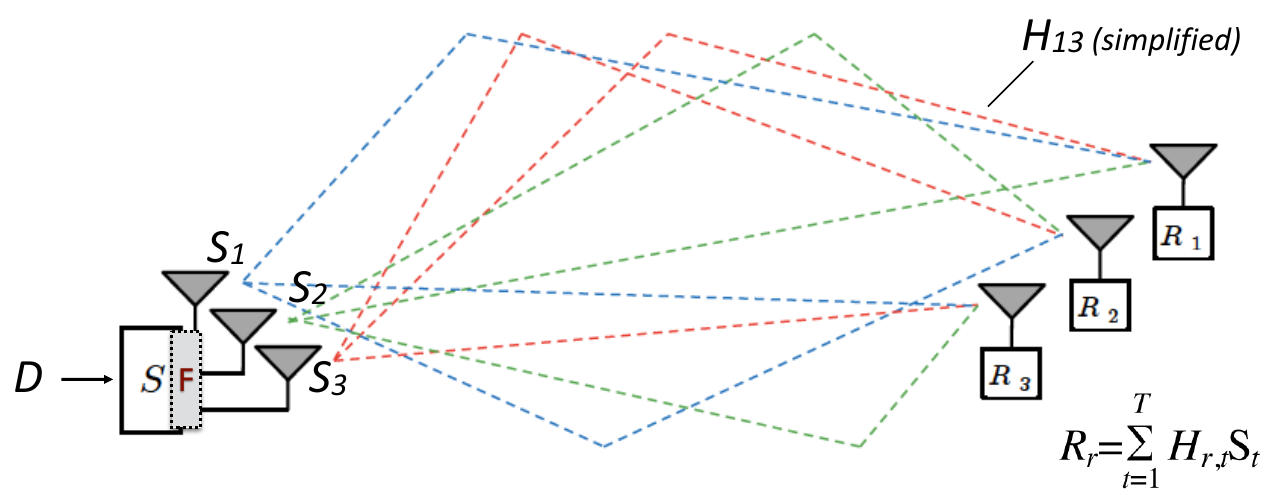
\includegraphics[scale=0.3]{images/7-mimo.png}
	\caption{MIMO channel}
	\label{fig:mimo}
\end{figure}

\paragraph{Analysis}
\begin{itemize}
	\item[$\oplus$] Stronger guarantees than SISO (beam forming focusses energy on receiver, jamming interferes with attacker)
	\item[$\ominus$] Still no authentication
	\item[$\ominus$] Still no guarantees on environment
	\item[$\ominus$] Still questionable benefit over classic public-private-key
	 schemes
	\item[$\ominus$] Passive attack: known plaintext attack (attacker can train filter)
	\item[$\ominus$] Active attack: abuse lack of authentication
\end{itemize}


\subsection{Friendly Jamming for Confidentiality and Access Control}

\paragraph{Friendly Jamming}
Transmit noise that the receiver can subtract (assuming a shared secret -- possibly established with one of the earlier methods).%
\footnote{Note the difference to orthogonal blinding, which does not add noise to all channels but only to the null space of the receiver's channel.}
The attacker on the other hand cannot distinguish signal and noise.

Example: IMD Shield for implanted medical devices.

\paragraph{Analysis} (as claimed by the IMD Shield paper). \\
Let $DJ$ be the distance between the data and jamming antenna (of the sender).
If $DJ > \lambda/2$ then an attacker with two antennas can separate the two signals (multiple channels).
Furthermore, if $DJ >> \lambda/2$ then the attacker can use directional antennas for signal separation.
\\
Thus the only ``safe'' case is $DJ < \lambda/2$ (i.e. when channels from D to A and from J to A are highly correlated).

However, this does NOT hold:
a MIMO attacker can retrieve the data even when $DJ < \lambda/2$, see the following:

\paragraph{Attack in Line of Sight LOS Model} 
The attacker places two antennas $A, B$ (see \autoref{fig:friendly-jamming-attack}).
The ideal placement is such that they receive both the jamming signal simultaneously (e.g. equidistant to the jammer) and the data signals with a phase shift of $\lambda/2$.
However, even with imperfect placement some data can still be recovered (with some attenuation).

When we also consider multipath effects (additional changes in amplitude and phase offsets) the attack becomes much harder.

\begin{figure}
	\centering
	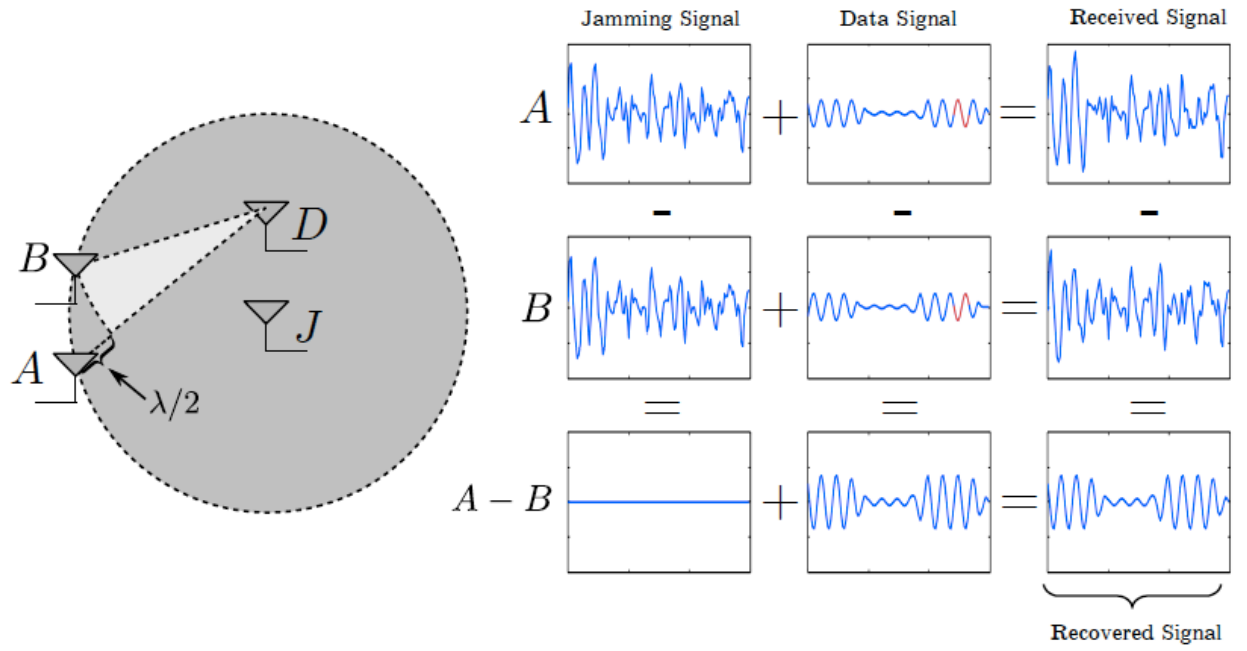
\includegraphics[scale=0.4]{images/7-friendly-jamming-attack.png}
	\caption{Friendly Jamming Attack Through Antenna Placement}
	\label{fig:friendly-jamming-attack}
\end{figure}

\paragraph{Conclusion}
Jamming works well for access control (in the sense that $J$ prevents malicious signals being send to $D$).
It does NOT work for confidentiality since a MIMO attacker can retrieve data even when $DJ < \lambda/2$.

In other words, the IMD Shield protects against malicious commands being sent to the implant, but not against an attacker listening to outgoing signals.

\paragraph{Signal Annihilation}
An attacker can deliberately introduce destructive interference to attenuate a legitimate signal.

Note that this is different to jamming!
Here, we are fooling the receiver to believe that there is \underline{no} signal on the channel.

\paragraph{Summary}
\begin{itemize}
	\item Using the physical layer for access control seems realistic.
	\item Using it for confidentiality however is questionable!
	Weak guarantees, use only as complementary measures.
\end{itemize}


\subsection{Broadcast Authentication: Presence Awareness}

\paragraph{Scenario}
One broadcasting station, many receivers.
No pre-shared keys, no credentials (certificates, public keys, etc).
Receivers know that they are within the power range of the legitimate sender 
(reasonable in airports, universities, etc).
Receivers know which channel (frequency) the sender is broadcasting.
The sender is always on and transmitting.

\underline{Goal}: distinguish between broadcast messages of legitimate and malicious station.
In other words, a physical layer-based broadcast authentication scheme based on presence awareness.
See also \autoref{sec:broadcast-auth}.

\paragraph{Integrity Codes Protocol} \mbox{}\\
\underline{Sender:}
Spread message $m$ from $k$ to $2k$ bits using Manchester encoding (1 $\rightarrow$ 10, 0 $\rightarrow$ 01).
Transmit result using on-off keying.
\\
\underline{Receiver:}
Set power thresholds above which to interpret a signal as 1. Then decode.
\\
\underline{Integrity Verification:}
Check if hamming weight%
\footnote{Recall that the hamming weight is the number of bits unequal to 0.}
$H(m)=|m|/2$. If yes, the message was not modified.

\begin{figure}
	\centering
	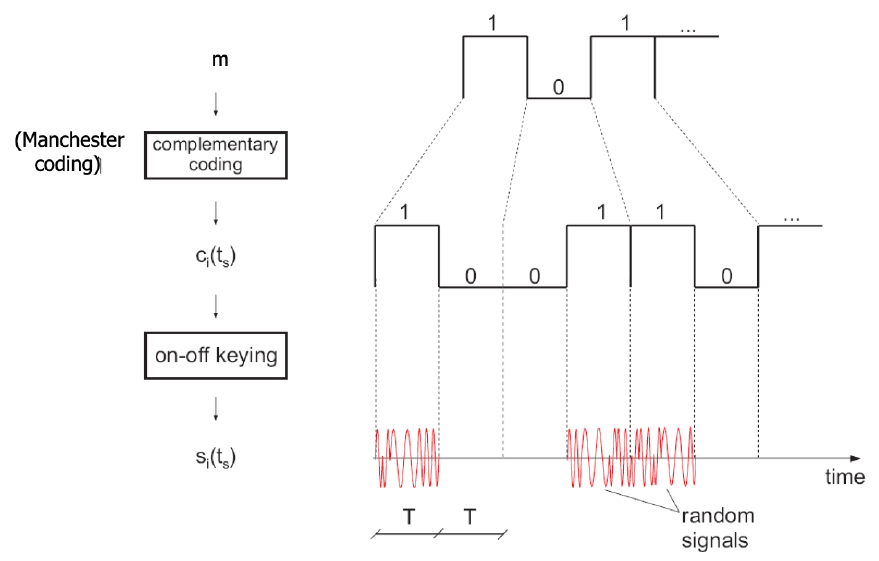
\includegraphics[scale=0.4]{images/7-integrity-code.png}
	\caption{Integrity Codes}
	\label{fig:integrity-code}
\end{figure}

\paragraph{Analysis}
\begin{itemize}
	\item The attacker can easily change $0 \rightarrow 1$ in the raw/keyed signal.
	They can change $1 \rightarrow 0$ only with small probability (assuming signal annihilation is hard).%
	\footnote{thgoebel: Why is this so? Just a couple of slides ahead it was explained that signal annihilation is doable?}
	\item How to handle arbitrary length messages?
	Solution: Use i-delimiters between messages. In Manchester encoding e.g. 111000.
	\item Slow. Solution: broadcast hash of message using integrity codes, use another faster channel for the full message.
\end{itemize}


\newpage

\section{Broadcast Authentication and Device Pairing}


\subsection{Broadcast Authentication: Delayed Key Disclosure} \label{sec:broadcast-auth}

\paragraph{Scenario}
One sender, many unknown (possibly malicious) receivers.
All (legitimate) receivers need to verify the authenticity of the broadcast messages.

\underline{Challenge:}
don't use public key cryptography (computationally expensive, especially on low-power devices), but instead only rely on symmetric cryptography.

\paragraph{One-way hash chain}
Repeated application of a hash function $F$, starting at an original value $s_l$ (see \autoref{fig:hash-chain}).
Due to the one-way property of hash functions an attacker knowing $s_i$ can only compute the subsequent value in the chain ($s_{i-1}$) but not the value $s_{i+1}$ that generated $s_i$.
This allows us to ``use'' the values $s_i$ one-by-one and always reveal a single new value.
See also Merkle hash trees.

\begin{figure}
	\centering
	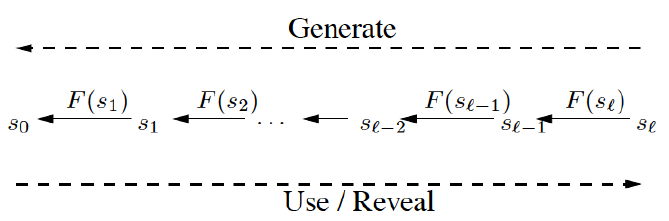
\includegraphics[scale=0.5]{images/8-hash-chain.png}
	\caption{One-way Hash Chain}
	\label{fig:hash-chain}
\end{figure}

\paragraph{Delayed Key Disclosure (TESLA)}
See \autoref{fig:tesla}.
\begin{itemize}
	\item The sender randomly generates a secret $K_l$, computes the entire hash chain and distributes $K_0$ as a ``public key'' to all receivers.
	\item To send a message $M_j$ in the interval $i$, it sends
	$$ P_j = \{ M_j || MAC(K'_i, M_j) || K_{i-d} \} $$
	where $||$ denotes concatenation and usually $d=1$.
	Note that we can send multiple messages in the same time interval using the same key.
	\item To verify a message, the receiver needs to receive $M_j$ and -- at a later time step and in another message -- the key $K_i$.
	They can then compute $K'_j$.\footnote{Why this extra hashing step is needed is ``an implementation detail''.}
	\\
	Then the receivers verify whether the MAC matches and the key $K_i$ does correctly hash down to the pre-loaded $K_0$ and whether the message was received in an interval where the key was valid.
	\item If a key is used after the interval, the message is ignored.
\end{itemize}

\underline{Analysis:}\\
TESLA achieves asymmetry by delaying the explicit disclosure of the self-authenticating keys in cleartext.
It requires time to be loosely synchronised between the sender and receivers.

\begin{figure}
	\centering
	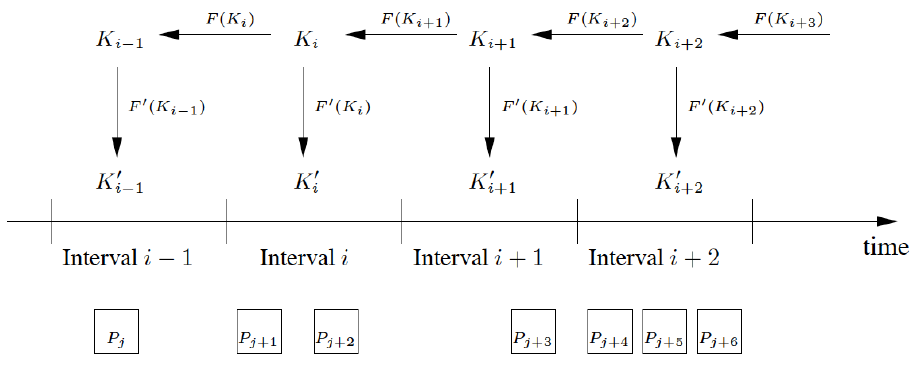
\includegraphics[scale=0.6]{images/8-tesla.png}
	\caption{TESLA}
	\label{fig:tesla}
\end{figure}



\subsection{Device Pairing}

\paragraph{Scenario}
We want to establish a secret key between two wireless devices, in the presence of an adversary.

\paragraph{Diffie-Hellman Key Exchange}
The classic secret key establishment scheme, established a shared key $k_{AB} = g^{ab} \mod p$.
See \autoref{fig:diffie} for a refresher.%
\footnote{We have prime $p$, a generator $g$ of $Z^*_p$ and the Diffie-Hellman assumption stating that the discrete logarithm is hard in some groups.}
However, it is only secure against a passive adversary:
an active attacker can trivially MITM the key exchange.

\underline{Goal:} Authenticate the DH key exchange between two wireless devices, to ensure they have established the same key.

\begin{figure}
	\centering
	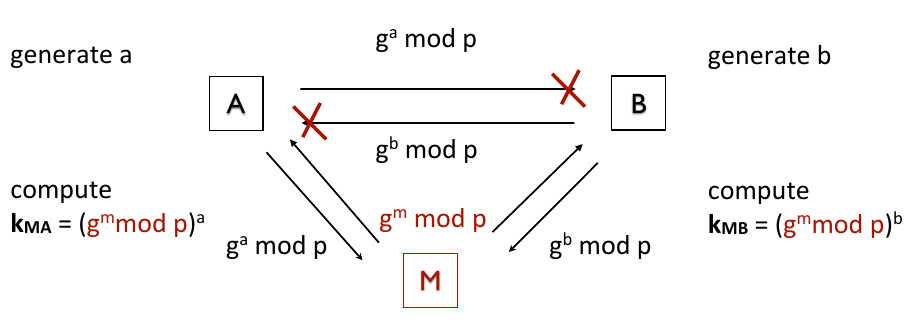
\includegraphics[scale=0.45]{images/8-diffie.png}
	\caption{Diffie-Hellman Key Exchange and MITM Attack}
	\label{fig:diffie}
\end{figure}

\paragraph{Device Pairing Proposals}
A selection:
\begin{itemize}
	\item Short string comparison: hash the key, display the string on both devices.
	\item Seeing is Believing: One device scans a QR code of the other's public key (one-way authentication).
	\item Load and Clear: has public key, map it to a recognisable sentence, read it out loud (text-to-speech TTS).
	\item Integrity Regions: use distance bounding to authenticate the key if the devices are in close proximity.
	\item Resurrecting duckling: first to receive the key becomes the owner for life.
	\item Shake them up: see below.
	\item PIN/Passkey entry: Bluetooth.
\end{itemize}

Note the different security assumptions:
only friends can be close, trust on first use, trusting the human, binding the success of the authentication to the happening and success of authentication (eliminating human error).

\paragraph{Shake them up} \mbox{} \\
\underline{Idea:} \\
Divide time into $N$ slots.
In each slot, randomly either $A$ or $B$ transmit a message.
A message is either 1 (``I am Alice'') or 0 (``I am Bob'').
Depending on who sent the message, this statement is either true or false.
Of course, both Alice and Bob know which is the case.
If the statement is true, set the next bit-to-be-exchanged to 1 otherwise to 0, thus creating a shared secret.
\\
Synchronisation and key exchange are initiated through physically shaking the device (hence the name).

\underline{Analysis:} \\
Assumes that Eve is too far away to distinguish messages from A and B, and can thus not know whether a statement was true or false.
This assumption may NOT hold as it can be attacked using signal fingerprinting to distinguish the source of a signal.
\\
Eve can insert messages, but then A and B will set their bits to different values (since none sent the message and will assume a false statement), thus only creating a DoS situation.

\begin{figure}[h]
	\centering
	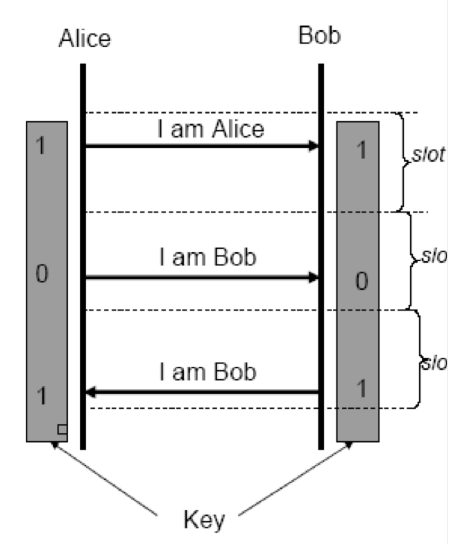
\includegraphics[scale=0.45]{images/8-shake.png}
	\caption{Shake Them Up}
	\label{fig:shake}
\end{figure}


\newpage

\section{WiFi Security}


\subsection{WiFi Basics}

\paragraph{Terminology}
\begin{itemize}
	\item \textit{Station (STA)/client}: terminal with access to the wireless media
	\item \textit{Access Point (AP)}: Station integrated both with the wireless media and the distribution system
	\item \textit{Service set/extended service set ESS}: Group of nodes logically grouped together and identified by their SSID
	\item \textit{Basic service set (BSS)}: Subgroups of a service set using the same radio frequency/the same AP (or in general: the same physical layer medium access means).
	\item \textit{Service set identifier (SSID)}: 32 byte name (usually human-readable) to identify a network
	\item \textit{Channel}: 20 MHz wide frequency range to use for WiFi, typically around 2.4 GHz and 5 GHz (see \autoref{fig:wifi-channels}).
	\item \textit{Medium Access Control (MAC)}: Goal: deliver data reliably and securely while sharing the open medium
\end{itemize}

\begin{figure}[h]
	\centering
	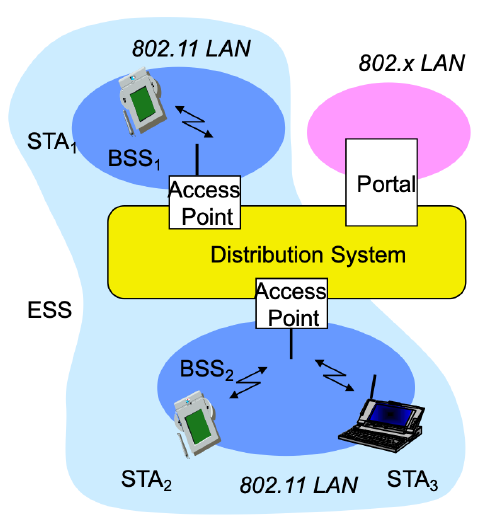
\includegraphics[scale=0.5]{images/9-wifi-terminology.png}
	\caption{WiFi System}%
	\label{fig:wifi-terminology}
\end{figure}

\begin{figure}[h]
	\centering
	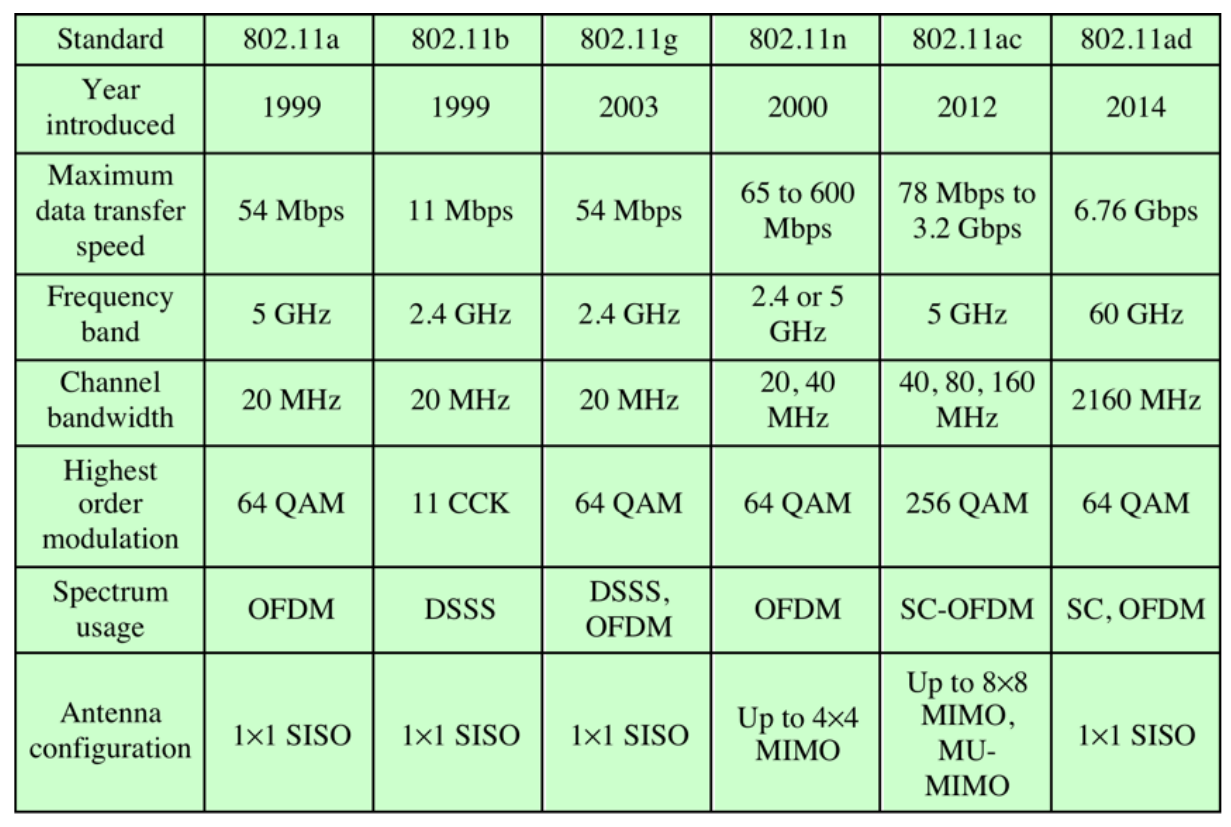
\includegraphics[scale=0.4]{images/9-wifi-versions.png}
	\caption{WiFi Standard Versions}%
	\label{fig:wifi-versions}
\end{figure}

\paragraph{Carrier-Sense Multiple Access with Collision Avoidance CSMA/CA}
Medium access control mechanism.
Part of the \textit{Distributed Coordination Function DCF}.
\begin{enumerate}
	\item \textit{Carrier sense} --- monitor medium to check if it is idle
	\item \textit{Collision avoidance} --- if another node sends, wait for a randomised \textit{backoff period}, then listen again
	\item \textit{Transmit} --- send entire frame, wait for ACK, if no ACK then backoff and wait
\end{enumerate}

\paragraph{Hidden terminal problem}
Occurs if a node B can communicate with two nodes A, C that cannot communicate with each other.
That is, if they both tried to send data to B they would individually sense the medium to be idle, but then they would clash at B anyway.
See \autoref{fig:hidden-terminal}.

The solution is to send a \textit{Request-to-Send RTS} message before transmitting a frame and wait for all nodes to reply with a \textit{Clear-to-Send CTS}.
Now when A sends a RTS even though C does not receive it, C still receives the CTS from B and will thus back off.
\\
This feature is optional in IEEE 802.11!

\begin{figure}[h]
	\centering
	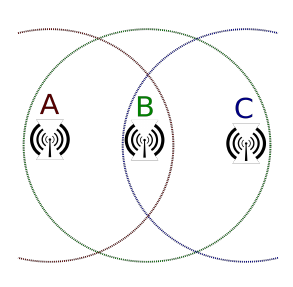
\includegraphics[scale=0.6]{images/9-hidden-terminal.png}
	\caption{Hidden Terminal Problem}%
	\label{fig:hidden-terminal}
\end{figure}

\paragraph{Frame types}
Data frames (user traffic), control frames (ACK, RTS/CTS), management frames (beacon\footnote{Contains basic information about the network, e.g. SSID, FH parameters, DSSS parameters, other supported options.}, association request, deauthentication).


\subsection{Basic Manipulations}

\paragraph{Capturing all frames}
Easy --- just install any packet capture software (such as Wireshark) and set the wireless interface to ``promiscuous mode''.

\paragraph{Communication (un)fairness}
DCF is fair --- assuming all stations adhere to it!
However by modifying backoff parameters in the wireless driver one can behave selfishly to get a higher throughput.

\paragraph{Jamming} \mbox{} \\
\underline{Simple:} \\
(a) Trigger carrier sense of transmitter (prevent sending, less power). \\
(b) Mangle the frame at the receiver (prevent receiving, more power).

\underline{Selective:} \\
Listen, decode prefix of an incoming frame and based on recipient address decide whether to jam the remaining data portion of the frame.
One needs to be very fast!

\paragraph{Man-in-the-middle}
Clone real AP onto different channel
$\rightarrow$ get clients to sign up to yours (e.g. jam real AP, send a Channel Switch Announcement CSA)
$\rightarrow$ inspect/manipulate/forward frames to real AP
$\rightarrow$ profit.


\subsection{WiFi Security Standards}

\subsubsection*{Wired Equivalent Privacy WEP}

First WiFi security standard (1997), with the goal of making wireless as secure as wired networks.
Today fully broken.

\underline{Operation:}\\
Checksum: plaintext $P = (m, CRC(m))$ \\
Encryption: ciphertext $C = P \oplus RC4(IV, k)$ (stream cipher RC4 with shared key $k$, initialisation vector $IV$) \\
Transmit $(IV, C)$.

\underline{Problems:}
\begin{itemize}
	\item \textit{Confidentiality}:
	Keystream reuse allows recovery of plaintexts:
	$$ C_1 \oplus C_2 = (P_1 \oplus RC4(IV,k)) \oplus (P_2 \oplus RC4(IV,k)) = P_1 \oplus P_2 $$
	Since the IV has 24 bits, at a data rate of 5 Mbps it will repeat after $\approx$ half a day.
	Knowing one of the plaintexts is reasonable (common structures such as IP headers, packet injection from the internet, other redundancies).
	\item \textit{Integrity}: CRC-32 is not a cryptographic MAC.
	This allows controlled message modification, i.e. given a $(ciphertext, checksum)$ pair we can create another $(ciphertext', checksum')$ pair such that the checksum is valid for the decrypted $plaintext'$.
	\item \textit{Access control}: works as follows:
	\begin{enumerate}
		\item AP sends a plaintext challenge
		\item Station replies with WEP encryption of challenge (proving possession of the key)
		\item AP completes association request
	\end{enumerate}
	Through simple traffic capture an adversary can learn a valid plaintext/ciphertext pair.
	From that they can derive the keystream to later compute a valid response to a new challenge (since the station can chose the IV).
\end{itemize}
Since 2007, tools like aircrack-ng allow recovering WEP keys in a matter of minutes.
\\
Wrong idea during design: ``in-flight'' modification of packets may be hard, but don't forget the possibility of offline attacks!


\subsubsection*{WiFi Protected Access WPA / Temporal Key Integrity Protocol TKIP}

Designed as a transitional mechanism in 2003 and to be compatible to WEP devices (though in 2019 still $\approx$ 50\% of networks accept it\dots).

\underline{Idea:}\\
Prevent keystream reuse and use a cryptographic MAC, while staying compatible to WEP.\@
``Achieved'' by augmenting encryption with per-packet key mixing, RC4 keystream filtering, a new integrity mechanism (MICHAEL) and counters for replay protection (TSC).
This allows to keep the WEP mechanism in hardware but change the inputs given to it.

\underline{ChopChop attack:} (for WEP!) \\
Capture an encrypted WEP frame.
Remove the last data byte, guess it, re-compute checksum for the shorter packet, use AP as an oracle (must discard frames whose checksums fail).
Rinse and repeat to learn one data block after the other.
\\
For a detailed explanation see \href{https://www.aircrack-ng.org/doku.php?id=chopchoptheory}{this aircrack doc entry}.
\\
Since this is a stream cipher, knowing one plaintext/ciphertext pair also reveals a keystream.

A similar attack also works for WPA/TKIP since MIC(HAEL) is reversible and the AP reports failures.

\underline{Biased keystream:} \\
There exist statistical biases in a RC4 keystream.
With enough packets this can be used to recover the plaintext for one MIC key.
Computationally expensive, but shows that crypto can be attacked, too.

\underline{Summary:}\\
Difficult start (had to reuse WEP hardware).
Raised the bar (despite ugly fix), but attacked in 2009, 2014/2015.
Okayish transition mechanism.


\subsubsection*{WPA2}

Introduced in 2004.
Better encryption (AES-128) and integrity (CBC-MAC, using \textit{authenticate-then-encrypt}).
Better authentication with a 4-way handshake.

\underline{Handshake:}\\
Goal: Starting from a \textit{Pairwise Master Key PMK} (that is derived from a shared passphrase) provide mutual authentication and establish a session key (\textit{Pairwise Transient Key PTK}).
\\
Steps: exchange nonces (msg1,2), derive PTK using PMK + nonces + MAC addresses, authenticate exchange (msg3,4).
Note that in msg2+3 the \textit{Message Integrity Code MIC} is also transmitted (missing in \autoref{fig:wpa2-handshake}).
\\
Proven ``secure'' in 2005 (mutual authentication and password is not leaked).

\begin{figure}[h]
	\centering
	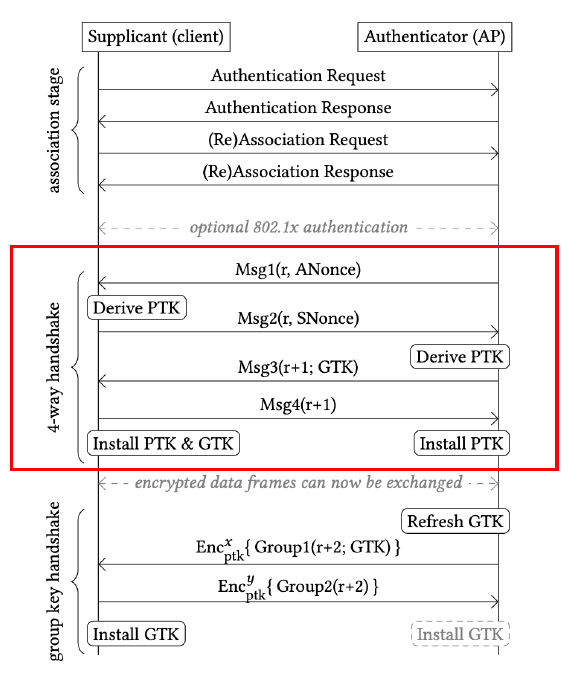
\includegraphics[scale=0.6]{images/9-wpa2-handshake.png}
	\caption{WPA2 Handshake}%
	\label{fig:wpa2-handshake}
\end{figure}

\underline{Dictionary attack}: \\
An adversary can capture the ANonce, SNonce and MIC.\@ \textit{If} the user chose a weak passphrase, then by brute force an attacker can try different passphrases, compute different PTKs and thus different MICs and compare the result to the captured MIC.\@

\href{https://www.krackattacks.com/}{\underline{Key Reinstallation Attack (KRACK)} (2017):} \\
Goal: force a keystream reuse.
\\
Observations: AP may retransmit msg3 if no ACK.\@ Each time, client reinstalls the \textit{same} PTK, and in the process it resets some counters.
This resulting in the same keystream being reused.
\\
Approach: Replay msg3.

\underline{Summary:}\\
Solid cryptography/encryption, weakness in handshake.
Proven properties hold, but model does not capture \textit{when} a key is installed.
Can be patched (and re-attacked).


\subsubsection*{WPA3}

Introduced in 2018.
Updated cryptography (AES-128/256 encryption, SHA-384 HMAC integrity), new handshake (based on the Dragonfly Key Exchange (\href{https://tools.ietf.org/html/rfc7664}{RFC 7664})).

\underline{Handshake improvements:}\\
Turns a low-entropy password into a high-entropy key, thus allowing for shorter passwords.
Has forward secrecy.

\href{https://wpa3.mathyvanhoef.com/}{\underline{Dragonblood} (2020):}\\
Transition mode allows downgrade to WPA2.
\\
Timing attack: execution time of turning the password into a group element at the start of the handshake depends on the password (i.e.\ a side-channel attack, though only for bad curves).


\newpage

\section{Cellular Security}


\subsection{1G: Analog}

\paragraph{Overview}
Introduced in the early 1980s to connect to the telephone network (\textit{Public Switched Telephone Network PSTN}).
Medium access control: split bandwidth with FDMA, with one call using the same frequency in both directions.
Suppprts handover between different base stations.

\paragraph{No security}
Identification via serial and phone numbers.
Control messages as analogue tones.

\underline{Problems:} eavesdropping (privacy), mobile cloning (billing fraud).


\subsection{2G: GSM}

\paragraph{Overview}
Introduced in the early 1990s.
Digital voice and control messages, enabling features like: compression, error correction, less power, SMS, security mechanisms.
We focus on the \textit{Global System for Mobile Communications GSM}.

\paragraph{Architecture}
See \autoref{fig:2g-arch}.

Medium access control: FDMA with distinct uplink/downlink frequency channels.
TDMA\footnote{Time-division multiple access} to support 8 speech channels on the same frequency.

Different channels for traffic and control frames (e.g. paging channel, random access channel, access grant channel).

\begin{figure}[h]
	\centering
	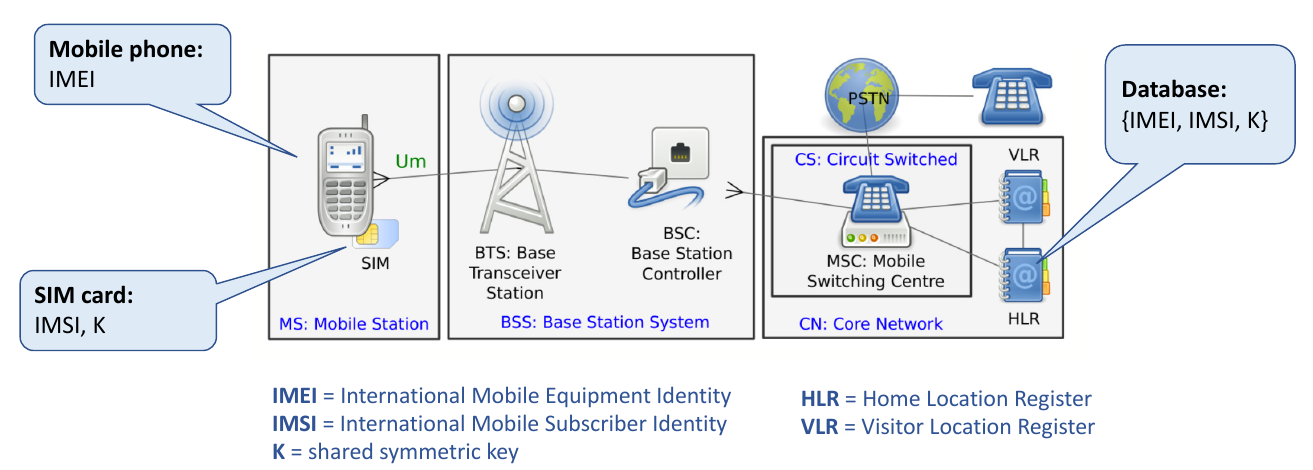
\includegraphics[scale=0.45]{images/10-2g-arch.png}
	\caption{Architecture of 2G}
	\label{fig:2g-arch}
\end{figure}

\begin{figure}
	\centering
	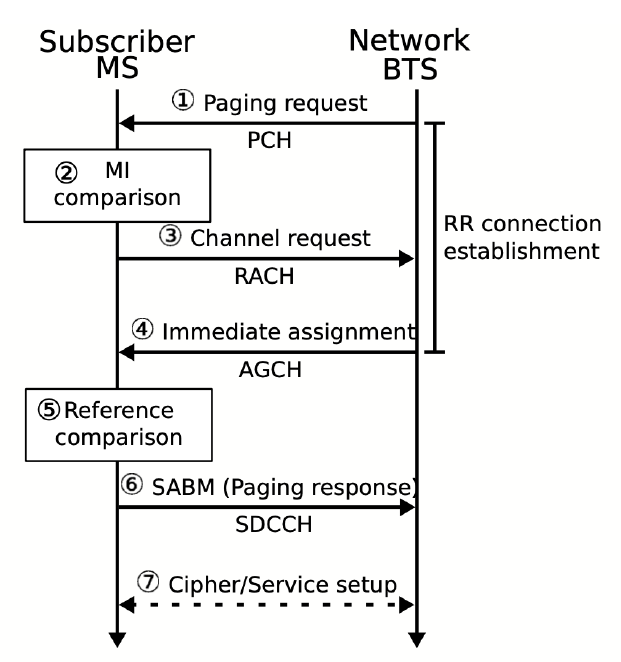
\includegraphics[scale=0.4]{images/10-2g-channels.png}
	\caption{Setup of incoming call (BTS ``pages'' the MS) over the different channels}
	\label{fig:2g-channels}
\end{figure}

\paragraph{Security model}
Everything based on symmetric shared keys $K_i$.
The key is stored in the \textit{Home Location Register HLR} of the provider and on the \textit{subscriber identification module SIM} card (and never leaves it).

\underline{Algorithms:}
A3 for authentication, A5 for encryption, A8 for key derivation.
Initially secret, but e.g. A5 leaked in the mid 90s, reverse engineered in 1999.

\paragraph{GSM authentication}
See \autoref{fig:2g-authentication}.
From the shared key $K_i$ and a random challenge a session key $K_c$ is derived.
Together with the frame nonce/counter $F_n$ it is used to encrypt the plaintext frame $m_i$.

Note that there is no mutual authentication (only the phone is authenticated) and messages can be replayed!
Also note that since A3 and A8 are executed on the SIM card, the operator can choose these!

\begin{figure}
	\centering
	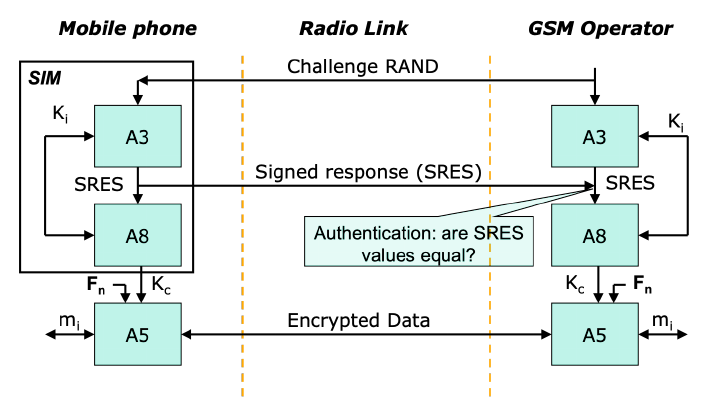
\includegraphics[scale=0.5]{images/10-2g-authentication.png}
	\caption{2G (Authentication) Flow}
	\label{fig:2g-authentication}
\end{figure}

\paragraph{GSM encryption}
Goal: fast in hardware.
Two variants A5/1 (strong) and A5/2 (weak, not discussed here).

\underline{A5/1:} stream cipher with a \textit{Linear Shift Feedback Register LSFR} and 64 bit security.
Registers are initialised with the key $K_c$ and the frame counter $F_n$ to create the keystream, which is then XORed with the plaintext.
See \href{https://web.archive.org/web/20120326211404/http:/l-system.net.pl/crypto/A5\_1\_stream\_cipher.svg}{here} for a visualisation of the LSFR.

\underline{Attack approach:} \\
Known plaintext/ciphertext pair
$\overset{XOR}{\longrightarrow}$ keystream
$\longrightarrow$ secret internal state
$\overset{solve\; LSE\; with\; 64\; eqns}{\longrightarrow}$ key

\begin{figure}
	\centering
	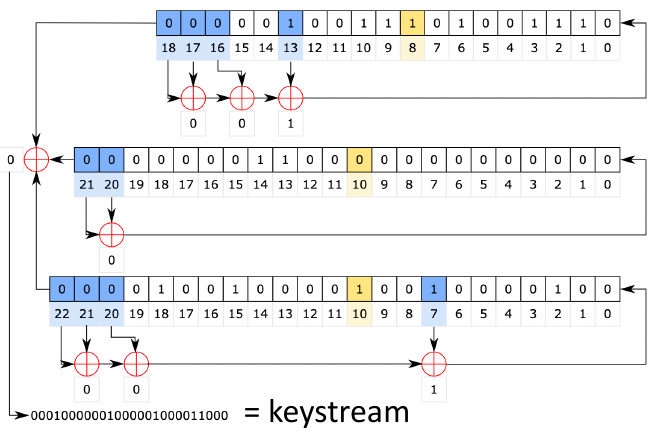
\includegraphics[scale=0.5]{images/10-2g-a5.png}
	\caption{2G A5 Linear Shift Feedback Registers}
	\label{fig:2g-a5}
\end{figure}

\paragraph{A5/1 attacks}
Attacks of A5/1 evolved over time (2000--2010).
The first were not very practical (requiring many known plaintexts or special-purpose hardware).
Types included: Time-Memory Tradeoff Attack (Biryukov 2000, Nohl 2010), Correlation Attack (Brakan \& Birham 2005), Guess and Determine Attack (Gendrullis et al. 2008), Fast Near Collisions (Zhang 2019).
\\
Note that a few known plaintexts are reasonable (known control frames).

\href{https://media.blackhat.com/bh-us-10/whitepapers/Nohl/BlackHat-USA-2010-Nohl-Attacking.Phone.Privacy-wp.pdf}{\underline{Karsten Nohl (2010):}}
2TB precomputed table (mapping from keys/state to keystreams, 1 month computation with 4 GPUs), 64 bit plaintext, 5 sec attack time (lookup).%
\footnote{Nohl omitted some attack details, later provided by Lu (2015).}
\\
Challenge: reducing table size ($2^{64}$ unreasonable).

\paragraph{Time-Memory Tradeoff Attack} (Hellman 1980)
\begin{enumerate}
	\item Precompute chains $x_1 \overset{f}{\rightarrow} x_2 \overset{f}{\rightarrow} x_3 \overset{f}{\rightarrow} ...$ where $f$ is A5/1.
	Store start point SP and end point EP.
	\item Attack: Create chain for the observed keystream.
	Check if any element in the chain matches a known EP.
	Re-create chain from SP to find the likely key (the element before the keystream in the re-computed chain).
\end{enumerate}
Tradeoff: longer chains mean less storage but more computation during the attack.

\begin{figure}
	\centering
	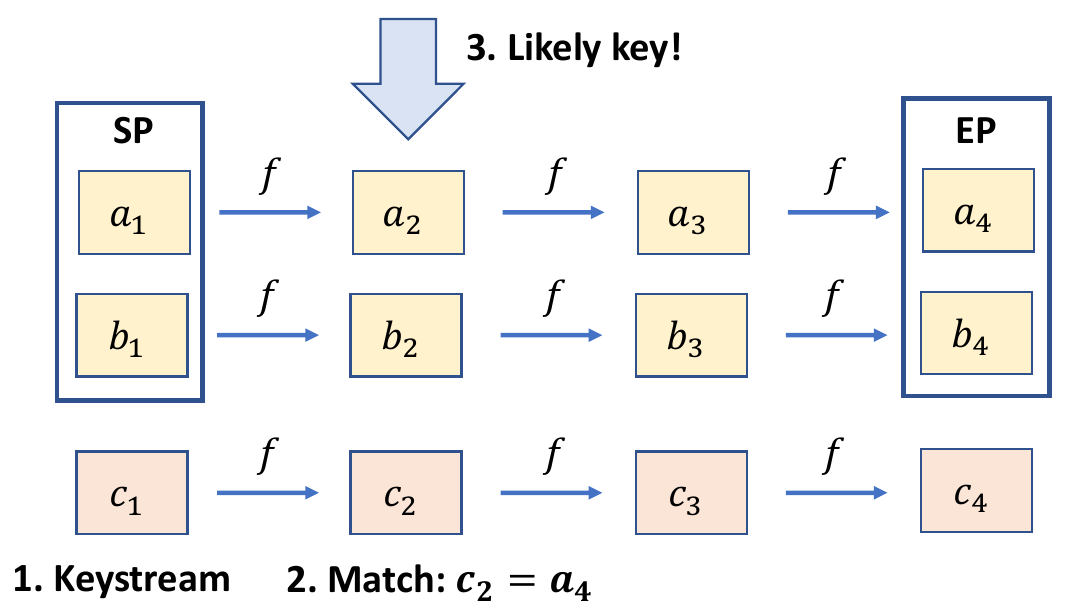
\includegraphics[scale=0.3]{images/10-2g-tmto.png}
	\caption{Time-Memory Tradeoff Attack}
	\label{fig:2g-tmto}
\end{figure}

\paragraph{Rainbow tables} (Oechslin 2003)
\\
Solves issue of collisions in chains (leading to reduced keyspace coverage as chains merge).
Uses different variant $f_i$ (``color'') for each chain link.
Different lookup details, but same idea.

\paragraph{A5/1 attacks summary}
Previous ideas generally applicable to stream ciphers, not just to A5/1.
Main enabler is the short key size (64 bit).
Nevertheless it lasted quite well considering when it was designed and under which hardware constraints, and given that there is still ongoing research.

\paragraph{A8 attacks}
Setup: $K_c$ known, want to recover $K_i$.
\\
1998: COMP128 hash inverted in hours (effectively only 54 bit)\\
2002: Faster recovery using side-channels.
\\
Mitigation: Operators replace A8 (OTA update, new SIM).

\paragraph{GSM -- no integrity protection}
No integrity protection defined, due to too much overhead (voice frame has 144 bits).
Also special use case: dropping frames/retransmission is undesired, and small voice frame modifications are acceptable.

\paragraph{GSM -- no mutual authentication}
Recall that the phone does not authenticate the base station.
Probable reasoning (1980s): expensive equipment, call encrypted anyway.
But: commercial fake BS (2000s), USRP (2010), etc enable user identification + tracking and MITM.


\subsection{SS7}

\paragraph{Signalling System 7 (SS7)}
Signalling network used in GSM + 3G to route calls, coordinate roaming, deliver SMS, etc.
Defined in the 80s/90s.

Initially only a few participating, mutually trusted operators.
But: Soon grew to 1000+ operators and third-party service providers, and SS7 access could be purchased at a low price.\\
$\implies$ Trust assumption violated.

Open source software and specs online, anybody with network access can send SS7 commands with a Linux computer.\\
$\implies$ Assumption on expensive equipment violated.

Attacks in 2014 by Engel (see the \href{https://media.ccc.de/v/31c3\_-\_6249\_-\_en\_-\_saal\_1\_-\_201412271715\_-\_ss7\_locate\_track\_manipulate\_-\_tobias\_engel}{31C3 talk here}), discussed below.

\begin{figure}
	\centering
	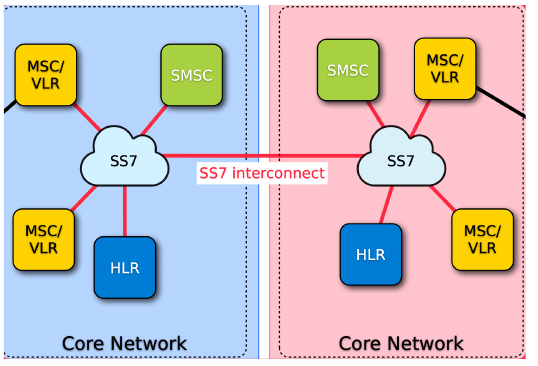
\includegraphics[scale=0.5]{images/10-ss7.png}
	\caption{SS7 Architecture}
	\label{fig:ss7}
\end{figure}

\paragraph{Location tracking}
Phone locations are stored in the \textit{Gateway Mobile Location Center GMLC}, access to which requires authentication (e.g. law enforcement).
However, by requesting the routing info from the HLR and with that the cell id from the \textit{Mobile Switching Center MSC} where the user is currently logged in, one can work around this to still get a rough location.

\begin{figure}
	\centering
	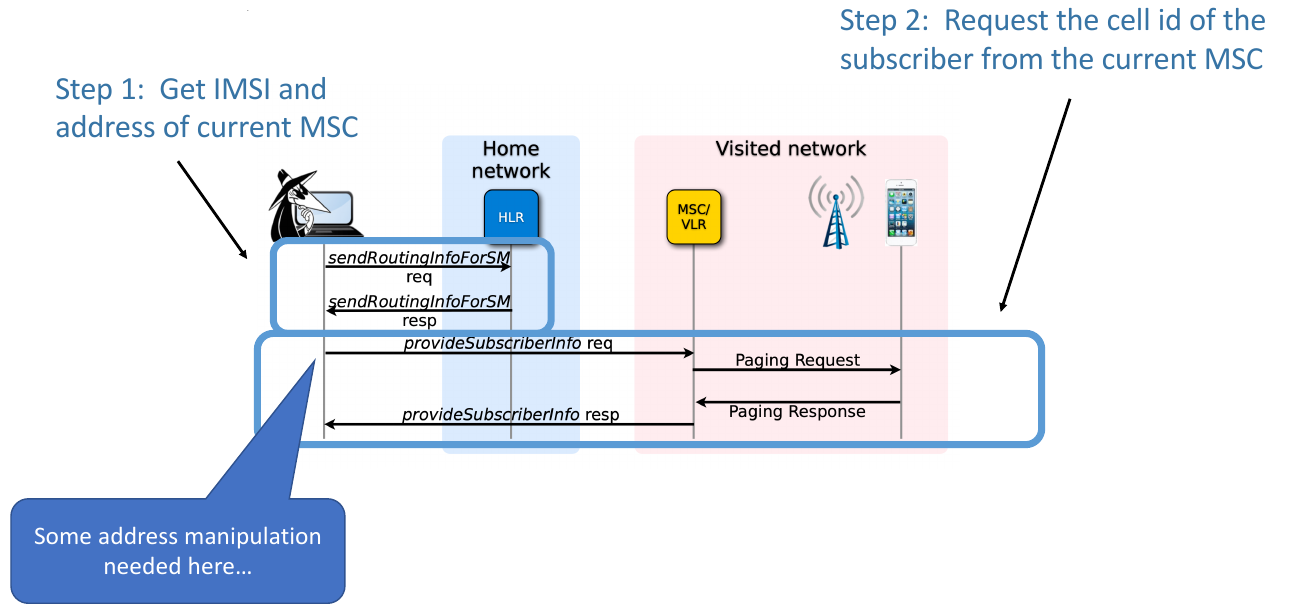
\includegraphics[scale=0.4]{images/10-ss7-location.png}
	\caption{SS7 Location Tracking}
	\label{fig:ss7-location}
\end{figure}

\paragraph{Intercepting Calls}
See \autoref{fig:ss7-calls}.
\begin{enumerate}
	\item Attacker overrides the \textit{GSM Service Control Function (gsmSCF)} in the MSC with their own.
	\item When the target makes a call, the MSC now contacts the attacker.
	\item The attacker learns the phone number and rewrites it towards their recording proxy.
	\item MSC sets up call to the proxy.
	\item Proxy bridges call to the intended receiver.
\end{enumerate}

\begin{figure}
	\centering
	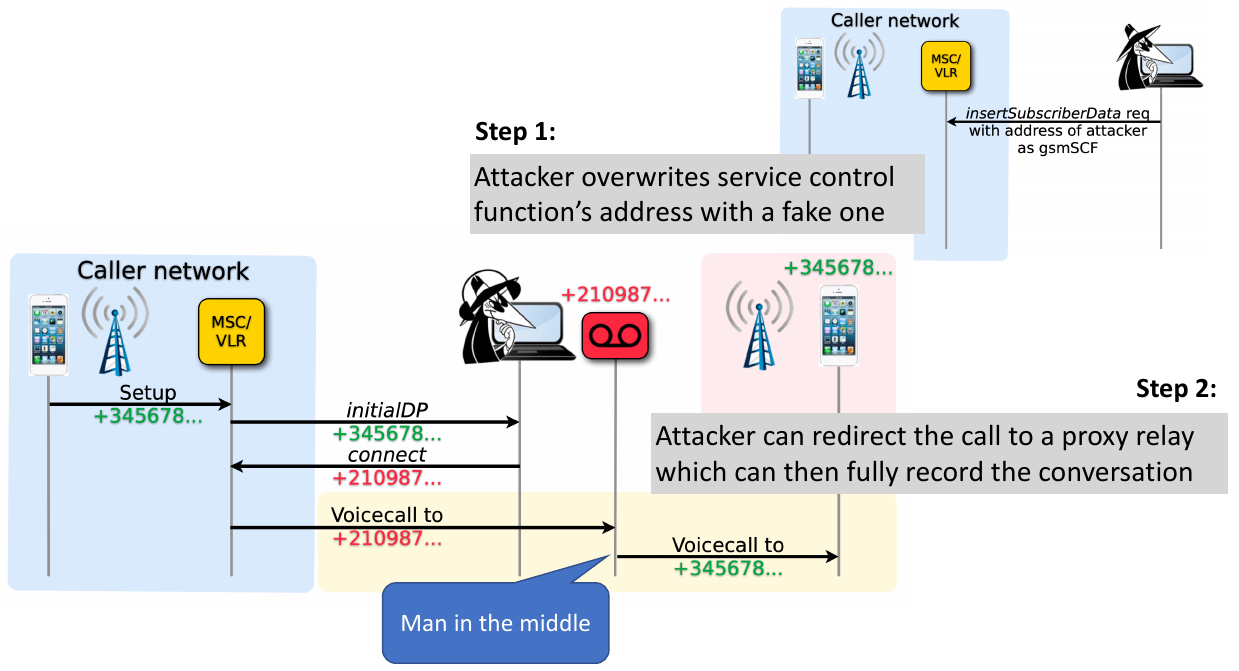
\includegraphics[scale=0.4]{images/10-ss7-calls.png}
	\caption{SS7 Intercepting Calls}
	\label{fig:ss7-calls}
\end{figure}

\paragraph{SS7 Summary}
Legacy system with outdated trust model.
Bad network management (open interfaces, no authentication or access control to control messages).
Attacks are independent of cryptography and the radio link (i.e. work from far away).
\\
Some issues were fixed, and LTE has a new signalling system (Diameter).


\subsection{3G: UMTS}

\paragraph{Overview}
\textit{Universal Mobile Telecommunication System UMTS} introduced in the early 2000s.

Radio link uses \textit{wideband code-division multiple access W-CDMA}, separate per-user spreading codes, distinct uplink and downlink frequency bands.

\paragraph{Protocol}
New \textbf{authentication and key agreement (AKA)} protocol.
Provides mutual authentication, mutual replay protection, integrity protection.
Also used in 4G+5G (more or less).

Similar design principles like GSM: operator and SIM trusted, phone and visited networks untrusted, minimise communication with home network.

\underline{Remarks:} (see \autoref{fig:3g-aka-details})
\begin{enumerate}
	\item Both the SIM card and the operator maintain the sequence number SQN (against replays)
	\item The IMSI\footnote{International Mobile Subscriber Identity} is send before the authentication (enabling tracking, see later)
	\item Function $f_1, f_2, f_3, f_4, f_5$ are operator-specific
	\item Loose synchronisation required
	\item Integrity key IK for integrity protection
\end{enumerate}

Further details on the authentication, encryption and integrity protection%
\footnote{Mandatory for signalling + control messages, optional for data. Based on a 8-round Feistel network to be fast in hardware.}
functions can be found in the slides but are omitted in this summary.

\begin{figure}
	\centering
	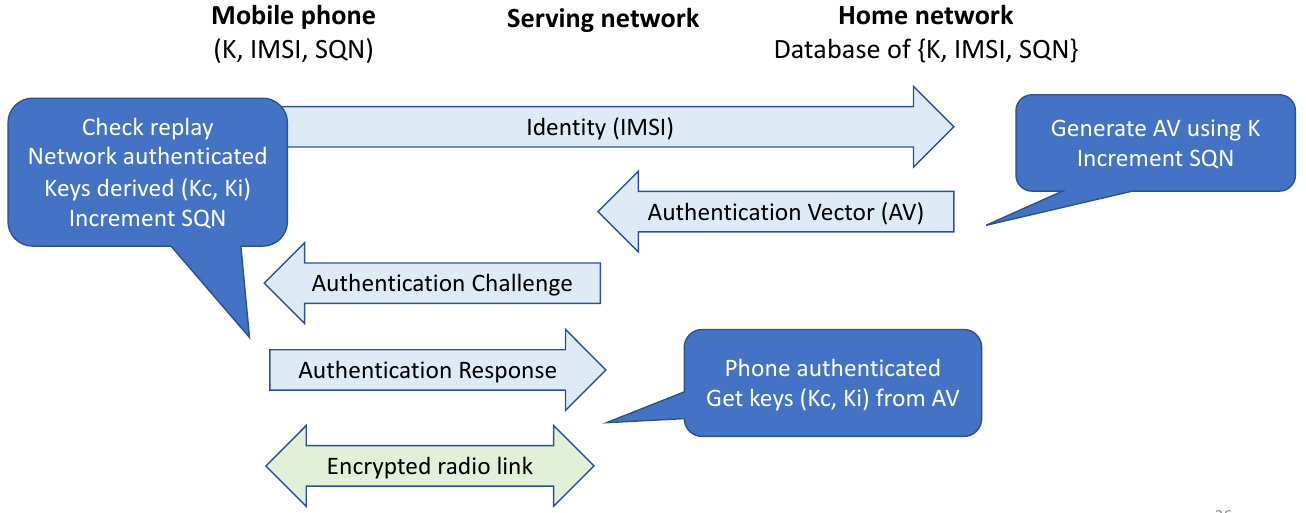
\includegraphics[scale=0.4]{images/10-3g-aka-overview.png}
	\caption{AKA High Level Flow}
	\label{fig:3g-aka-overview}
\end{figure}

\begin{figure}
	\centering
	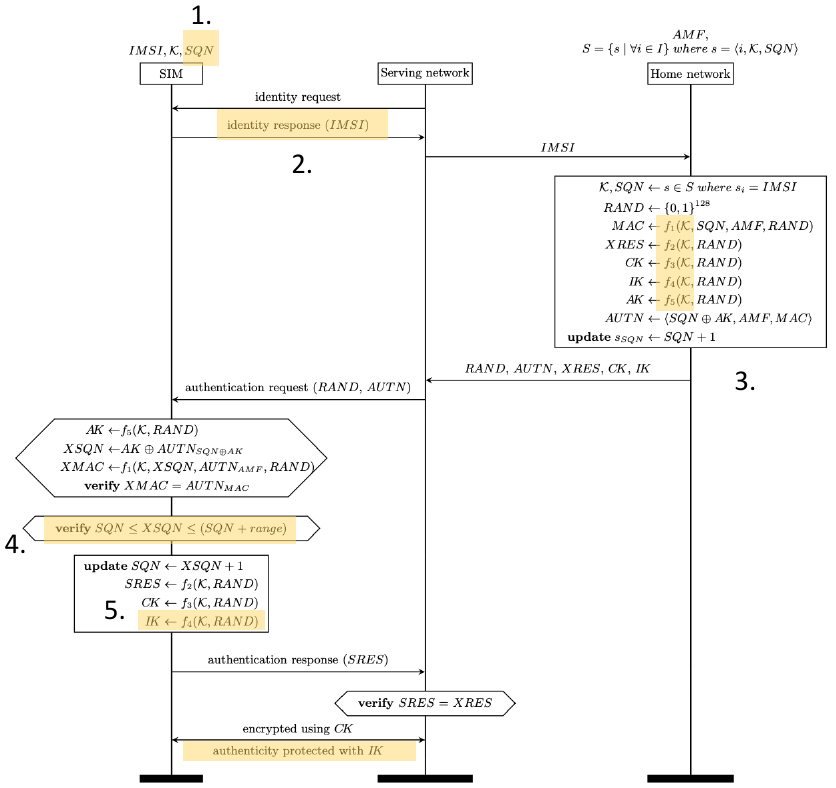
\includegraphics[scale=0.7]{images/10-3g-aka-details.png}
	\caption{AKA Detailed Flow}
	\label{fig:3g-aka-details}
\end{figure}

\paragraph{Cryptography Summary}
Authentication and Key Agreement protocol formally verified with respect to authentication and confidentiality (2001).
Two known but impractical attacks on encryption (interesting for research though).
TLDR: Good for now.

\paragraph{Denial of Service}
Commercial jammers available for a few hundred dollars (though use is illegal!).
\\
Approaches:
\begin{itemize}
	\item Insert noise on physical layer.
	\item Jam/block paging messages (control layer). Difficult, requires synchronisation with the victim.
	\item Answer paging messages faster than the victim, causing the victim's reply to be ignored.
	Possible because (a) paging occurs before authentication and (b) base stations cover large areas.
\end{itemize}

\paragraph{MITM/Fake BS}
Though AKA authentication is mutual, a MITM perform a downgrade attack to force the phone to use GSM (due to co-existence).
Also in 3G the MITM can learn the IMSI at the start of AKA.

\underline{Practical considerations:}
Which frequency to use -- allocated or unallocated?
What cell id to use -- a new, unknown one?
Jam legitimate BS to get victims to connect to yours?
\\
$\implies$ Though setting up a fake BS is easy, detecting it is easy as well.

\paragraph{Femtocells}
Operator provides a ``mini-BS'' to customers to improve local (indoor) coverage.
The femtocell box relays from the radio link to the operator network.

Vulnerable because they are easier to access then normal base stations (high up on a tower).
Gaining access gives a perfect MITM position, having the keys for the gateway to the operator as well as for the radio link.

\paragraph{User tracking}
Identity (IMSI) is sent before authentication.
Even though a temporary identity (IMSI) is issued, the IMSI is reused on occasions.
Thus user tracking is possible to some extent, but not addressed by the spec (tradeoff possibility of abuse versus increased complexity).

\underline{Approaches for identity protection}:
\begin{itemize}
	\item \textit{Pseudonyms}: send pseudonym when starting AKA, with the home network always returning a new pseudonym
	(encrypted\footnote{Note that this encryption can be done symmetrically with the shared key, since the home network could use the pseudonym to look it up.}, so that the serving network cannot read it).\\
	Challenge: requires synchronisation, and thus a recovery process.
	However, it is hard to design a recovery process that cannot be abused to learn the IMSI.
	\item \textit{Public key encryption}: store home network public key on SIM, encrypt IMSI.
	Defined as optional in 5G.
	Pro: no state that needs to be synchronised.
	Con: asymmetric cryptography is expensive.
\end{itemize}


\subsection{4G: LTE}

\paragraph{Overview}
\textit{Long-Term Evolution LTE} introduced in 2008.
\\
\underline{Updated architecture:}
fully packet switched, new core network (\textit{Evolved Packet Core EPC}, fully packet-switched), new radio network (\textit{Evolved UMTS Terrestrial Radio Access Network E-UTRAN}), but interoperable with legacy systems.
\\
\underline{Updated physical layer:}
\textit{Orthogonal Frequency Division Multiplexing OFDM} (downlink with orthogonal sub-carriers, single-carrier uplink), multiple antennas (MIMO).

\paragraph{Architecture and Terminology}
See \autoref{fig:4g-arch}.
\begin{itemize}
	\item \textit{User Equipment UE} (MS): the mobile handset
	\item \textit{Evolved Node B eNB} (BS): the base station
	\item \textit{Mobility Management Entity MME}: handles signalling via the \textit{Non-access stratum NAS}, UE authorisation, S-GW selection
	\item \textit{Home Subscriber Server HSS} (HLR): subscriber database, user authentication
	\item \textit{Serving Gateway S-GW}:  routes user data packets
	\item \textit{Packet Gateway P-GW}: connects to external network, routing, filtering
\end{itemize}

\begin{figure}
	\centering
	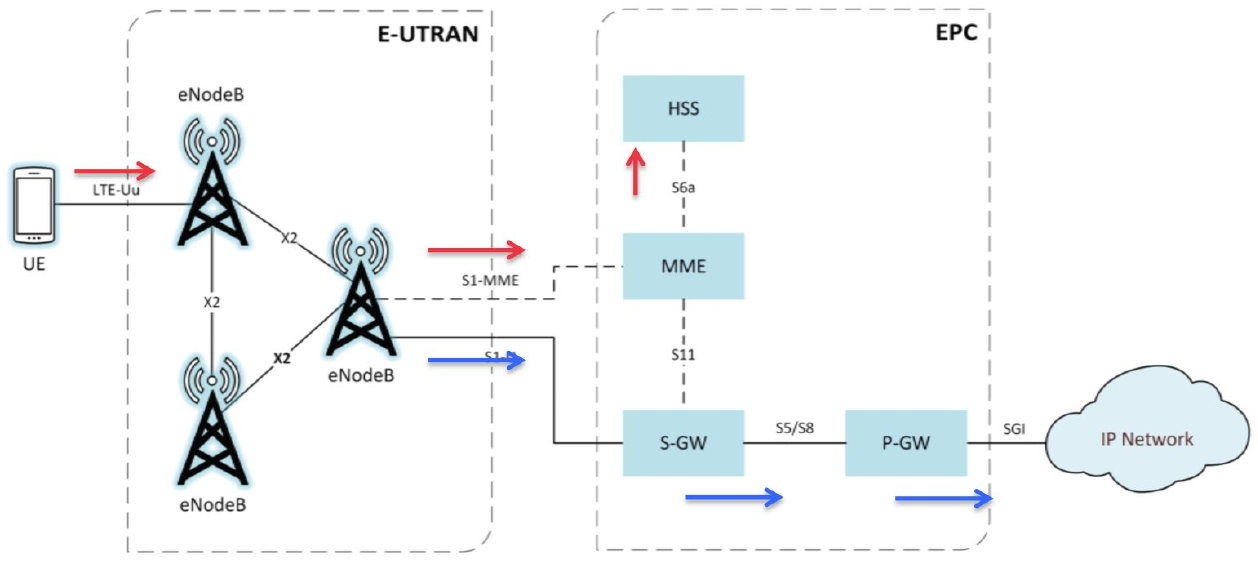
\includegraphics[scale=0.5]{images/10-4g-arch.png}
	\caption{LTE Architecture}
	\label{fig:4g-arch}
\end{figure}

\paragraph{Network Protocol Stack}
See \autoref{fig:4g-network-stack}. From top to bottom:
\begin{itemize}
	\item \textit{Non-access stratum NAS}: mobility management, tracking area update, etc
	\item \textit{Radio Resource Control RRC}: AKA, paging messages, system information broadcast, etc.
	\item \textit{Packet Data Convergence Protocol PDCP}: compression, optionally encryption+integrity
	\item \textit{Radio Link Control RLC}: error correction, segmentation, frame ordering
	\item \textit{MAC layer}: manages access to radio link
\end{itemize}
Note that everything below the PDCP layer is unencrypted.
Thus most sniffing+spoofing attacks focus on the layers below.

\begin{figure}
	\centering
	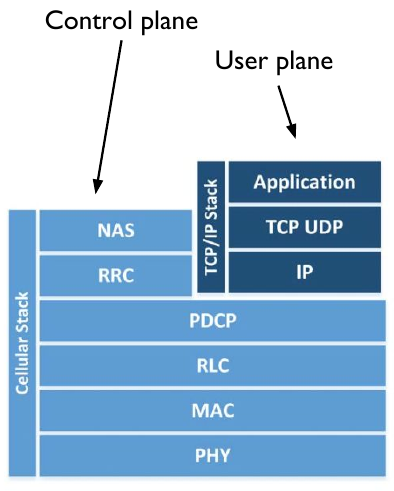
\includegraphics[scale=0.5]{images/10-4g-network-stack.png}
	\caption{LTE Network Protocol Stack}
	\label{fig:4g-network-stack}
\end{figure}

\paragraph{Security Overview}
Authentication: similar to AKA.

Encryption/integrity: 3 variants EEA1, EEA2, EEA3 and EIA1, EIA2, EIA3.

Other: extended key hierarchy, option for longer keys (256 bit), handover between eNBs (X2), backhaul (S1) protection.

\paragraph{Key hierarchy}
to limit attack possibilities and impact.
Master key $K$ (128 bits, stored on HSS+SIM), confidentiality key $CK$, integrity key $IK$, etc.
\begin{figure}
	\centering
	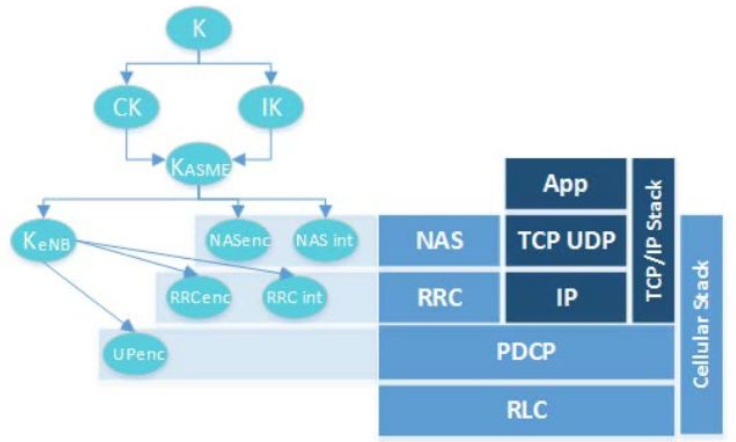
\includegraphics[scale=0.5]{images/10-4g-key-hierarchy.png}
	\caption{LTE Key Hierarchy}
	\label{fig:4g-key-hierarchy}
\end{figure}

\paragraph{Backhaul + EPC protection}
For backhaul, the LTE spec recommends physical protection.
For EPC, the spec is vague (``division of security domains'').
In practice both are secured using standard IP security practices (VPN, PKI).

\paragraph{Handover + Key Separation}
Reduced attack surface and key scope by limiting key lifetime of $K_{eNB}$.
E.g. different keys for different eNBs/cells.

\paragraph{Location tracking} \mbox{} \\
\underline{Background:}
The service area is divided intro \textit{tracking areas TAs} containing multiple cells (each controlled by an eNodeB that broadcasts information such as the TA code, mobile network code, cell ID).
UE sends IMSI with the Attach request, in which the operator assigns temporary identifiers that are used subsequently (TMSI, GUTI\footnote{Global unique temporary identifier}).

\underline{Adversary:}
Goal: learn user locations.
Capabilities: transmit/receiver radio signals, possible with commercial USRPs.
Advantage: GUTI re-allocation depends on operator, possibly not changed for multiple day.

\underline{Attack:}
\begin{enumerate}
	\item Set up fake BS.
	\item Monitor user presence in TA.
	\item Learn precise location:
	actively send unprotected \textit{RRC Connection Reconfig} messages, to which the UE responds with a \textit{Measurement Report} containing the signal strengths of neighbouring cells and its GPS location.
\end{enumerate}

\underline{Analysis:}
Not all signalling/control messages are integrity protected/authenticated.
Spec allows this explicitly for troubleshooting (availability versus privacy).

\paragraph{MITM} \mbox{} \\
\underline{Background:}
MAC layer assigns unique \textit{Radio Network Temporary Identifiers RNTIs} to distinguish UEs.
eNodeB uses \textit{Downlink Control Information DCI} to notify UEs when radio resources are available.
Also recall that EEA2 uses AES-CTR for encryption (XORs keystream with plaintext).

\underline{Attack:}
\begin{enumerate}
	\item Identify UE from encrypted traffic: observe connection establishment, learn TMSI+RNTI, use paging to map TMSI to phone number.
	\item Modify/redirect encrypted traffic: often uplink is encrypted but not integrity protected. Xor ciphertext with ``manipulation mask'' (try-and-error).
\end{enumerate}

\underline{Analysis:}
Identifiers on lower layers, encryption on higher layers.
Integrity protection optional.

\paragraph{Jamming/DoS}
Brute-force jamming always possible, but requires a lot of power.
Instead, targeting specific control channels can be effective, too (see next point).

\paragraph{Signal Overshadowing (SigOver)} \mbox{} \\
\underline{Idea:}
Broadcast signals are not integrity protected (e.g. \textit{System Information Blocks SIBs)}.
Spoof them by overshadowing specific frames of the legitimate broadcasts (providing a misconfiguration to prevent the UE from connecting).

\underline{Analysis:}
Low jamming-to-signal ratio (J/S), thus stealthy (not as obvious as a fake BS).
Only downlink affected, thus undetected by the base station.
Challenges: time+frequency synchronisation with the legitimate signal, distance/delay estimation to the UE, phone may quickly reconnect to another cell.

\underline{Commercial Mobile Alert Service CMAS} messages (``presidential alerts'') are also delivered via SIB12, allowing signal overshadowing.

\paragraph{Keystream Reuse Attack / ReVoLTE} \mbox{} \\
\underline{Idea:} IV for EEA comprised of a counter, radio bearer ID and radio direction.
\\
Unfortunately, many operators re-use bearer IDs and reset counter for subsequent calls (exactly what we need!).
Adversary can initiate a second call just after the target call and record both keystreams.
\\
Fix: don't repeat id and counter.

\paragraph{4G Summary}
New crypto algorithms, new core network.
Small security improvements (key hierarchy, handover protection), but not yet perfect.
\\
Types of attacks: SigOver, fake base stations, man-in-the-middle.
\\
Attack properties: stealthiness/detectability, power requirement, J/S ratio.


\subsection{5G}

\paragraph{Overview}
Currently being deployed (2019/2020).
\\
\underline{Radio link}: \textit{5G New Radio NR}, optimised OFDM, massive MIMO, two frequency ranges (FR1: sub-6GHz, FR2: mmWave range, 24-100GHz, high-throughput, high-bandwidth).
Beam management to steer beams with a phase array allows connecting more devices.
\\
\textit{Time Division Duplex TDD} allows the same channel/frequency to be used for both up- and downlink, with different time intervals for different directions.%
\footnote{Compare this with LTE which used FDD: the uplink and downlink used different frequencies.}
On one hand this allows flexible allocation, but on the other it requires precise synchronisation!

\paragraph{Attacks}
Some ideas as research is ongoing.
\begin{itemize}
	\item Beam stealing: attack beam training to steer beams away from victims (shown for IEEE 802.11ad)
	\item Broadband jamming (DoS): increasingly difficult due to large bandwidth (power constraint) $\implies$ need protocol-aware spoofing for DoS (challenge: tight synchronisation).
	\item PSS\footnote{Primary Synchronisation Signal} spoofing:
	soft takeover: synchronise to cell, introduce PSS at correct timing then slowly move peak away (see GNSS \autoref{sec:gps-spoof}).
\end{itemize}

\paragraph{5G Security Summary}
Similar crypto algorithms.
Better replay protection for AKA (SIM generates nonces).
User tracking mitigations (SIM can encrypt IMSI/TMSI with home operator's public key, stricter policies for changing temporary ids).

\begin{figure}[h]
	\centering
	\includegraphics[scale=0.5]{images/10-overview.png}
	\caption{Cellular Security Summary}
	\label{fig:overview}
\end{figure}


\newpage

%
% Appendix
%
\appendix

%\part{Appendix}

\section{Imprint}

This document closely follows the lecture slides of the \textit{Security of Wireless Networks} lecture in the autumn semester 2020 at ETH Zurich.
Our contribution to this is editing the whole lot and refactoring even more so that it may fit the "lecture summary" style.
However, basically all graphics are copy \& pasted from the slides. If you don't want yours here, please contact us and we will remove them.

In addition, this summary is based on a summary by Sarah Kamp.

Otherwise, our part of the work is published as CC BY-NC-SA.

%\begin{center}
%\ccbyncsa
%\end{center}


%\bibliographystyle{plain}
%\bibliography{references}

\end{document}